\documentclass[12pt]{article}
\usepackage{graphicx} % Required for inserting images
\graphicspath{{figures/}}
\usepackage{url}
\usepackage{float}
\usepackage{subcaption}
\usepackage{xurl}
\setlength{\parindent}{0pt}
\usepackage[
  margin=1in,
  headheight=12pt,   
  headsep=6pt        
]{geometry}

\title{Computer Vision Assignment}
\author{Mairead O'Dwyer}
\date{November 2026}

\begin{document}

\maketitle

Generative Artifical Intelligence (GenAI) was used in the assignment. Please see the AI declaration document for further detail.  
This is the GitHub repository link: \url{https://github.com/Mairead-1402/CV_Assignment}. 
\section{Theory of Processing}
\subsection{Detection of the pool balls}

The pool balls were detected using Hough Circle transform on the original, untransformed images as they are mainly circular in shape and transforming the image may make the balls appear more elliptical. 
Hough Circle requires greyscaled images as it focuses on the edges of the image rather than the colour. Each image was converted to greyscale before being smoothed [5]. 
Smoothing removes noise within the image and blurring some edges within the image. Guassian blurring was used as it blurs edges within the images [5]. This helps when trying to use Hough Circle transform on the pool balls as striped balls, when orientated in a certain way, can appear to have two circles within them, the circle of the ball and a white circle at the base or top of the ball. 
\begin{figure}[H]
    \centering
    \begin{minipage}[b]{0.48\textwidth}
        \centering
        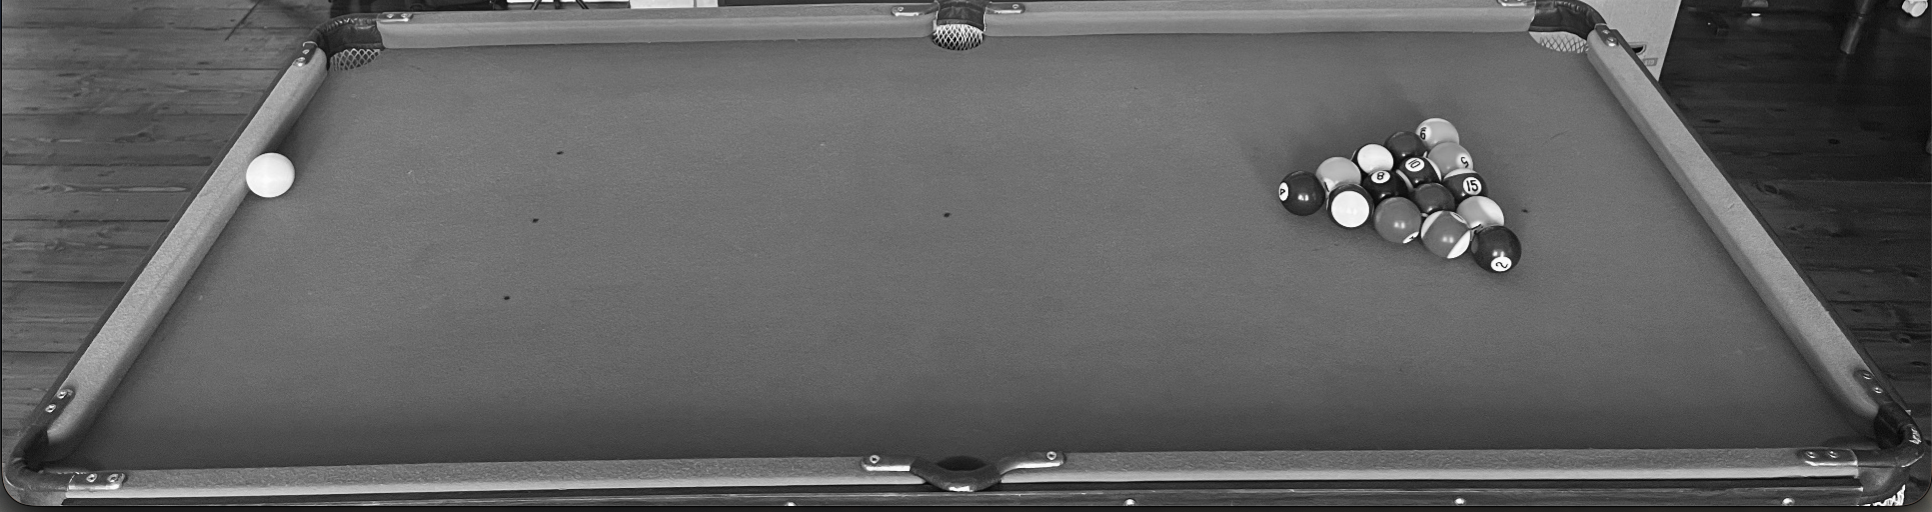
\includegraphics[
            width=\linewidth,
            height=3cm,
            keepaspectratio
       ]{figures/CV_Fig1.png} 
    \caption{Greyscale Image of Table1.jpeg}
        \label{fig:fig1}
    \end{minipage}
    \hfill
    \begin{minipage}[b]{0.48\textwidth}
        \centering
        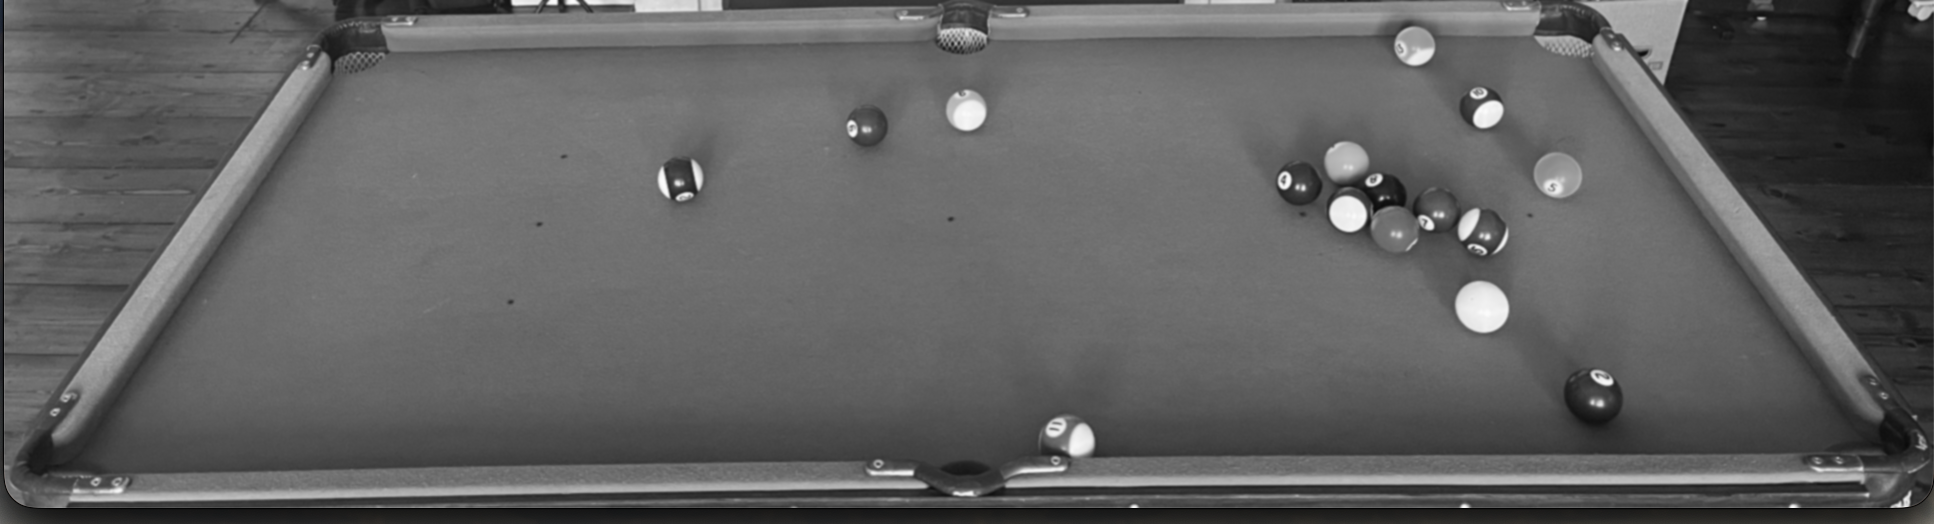
\includegraphics[
            width=\linewidth,
            height=5cm,
            keepaspectratio
        ]{figures/CV_Fig2.png}
        \caption{Guassian Blurring applied to greyscale image of Table2.jpeg}
        \label{fig:fig2}
    \end{minipage}
\end{figure}

Hough Circle Transform was applied within each image to find circles within the image [5]. However it requires parameter setting in order to not find every circular shape in the image. The transform requires 9 parameters: image, circles, method, dp, minDist, param1, param2, minRadius, maxRadius [1]. Parameters were chosen by selecting baseline parameters and altering them until a good level of accuracy was achieved. The parameters were tuned using the AllBalls.jpeg image. The dp parameter was set to 1 to keep the circles as the same resolution as the inputted image [1]. The minDist is the minimum distance between each centre of the ball. It was set to 25 as it allowed for instances where one ball would be behind another, and the former's centre could align with the former's edge. The param1 is the upper limit for the internal Canny detector.
65 was chosen as the upper limit, with $\approx 33$ for the lower limit. It gives a good detection accuracy as it allows for both weak edges and the defined circles of the balls. Param2 is the amount of evidence for a circle to be considered a ball.
15 was chosen as higher values missed balls in the detection. The final two parameters were the minimum radius and the maximum radius of the circles detected, respectively. The radius limits were set to 20 and 24. This allowed for circles to be detected in the background and the foreground while also attempting to keep false positives to a minimum. These parameters allow for a good detection accuracy but also results in balls not being detected and false predictions.

\begin{figure}[H]
    \centering
    \begin{minipage}[b]{0.48\textwidth}
        \centering
        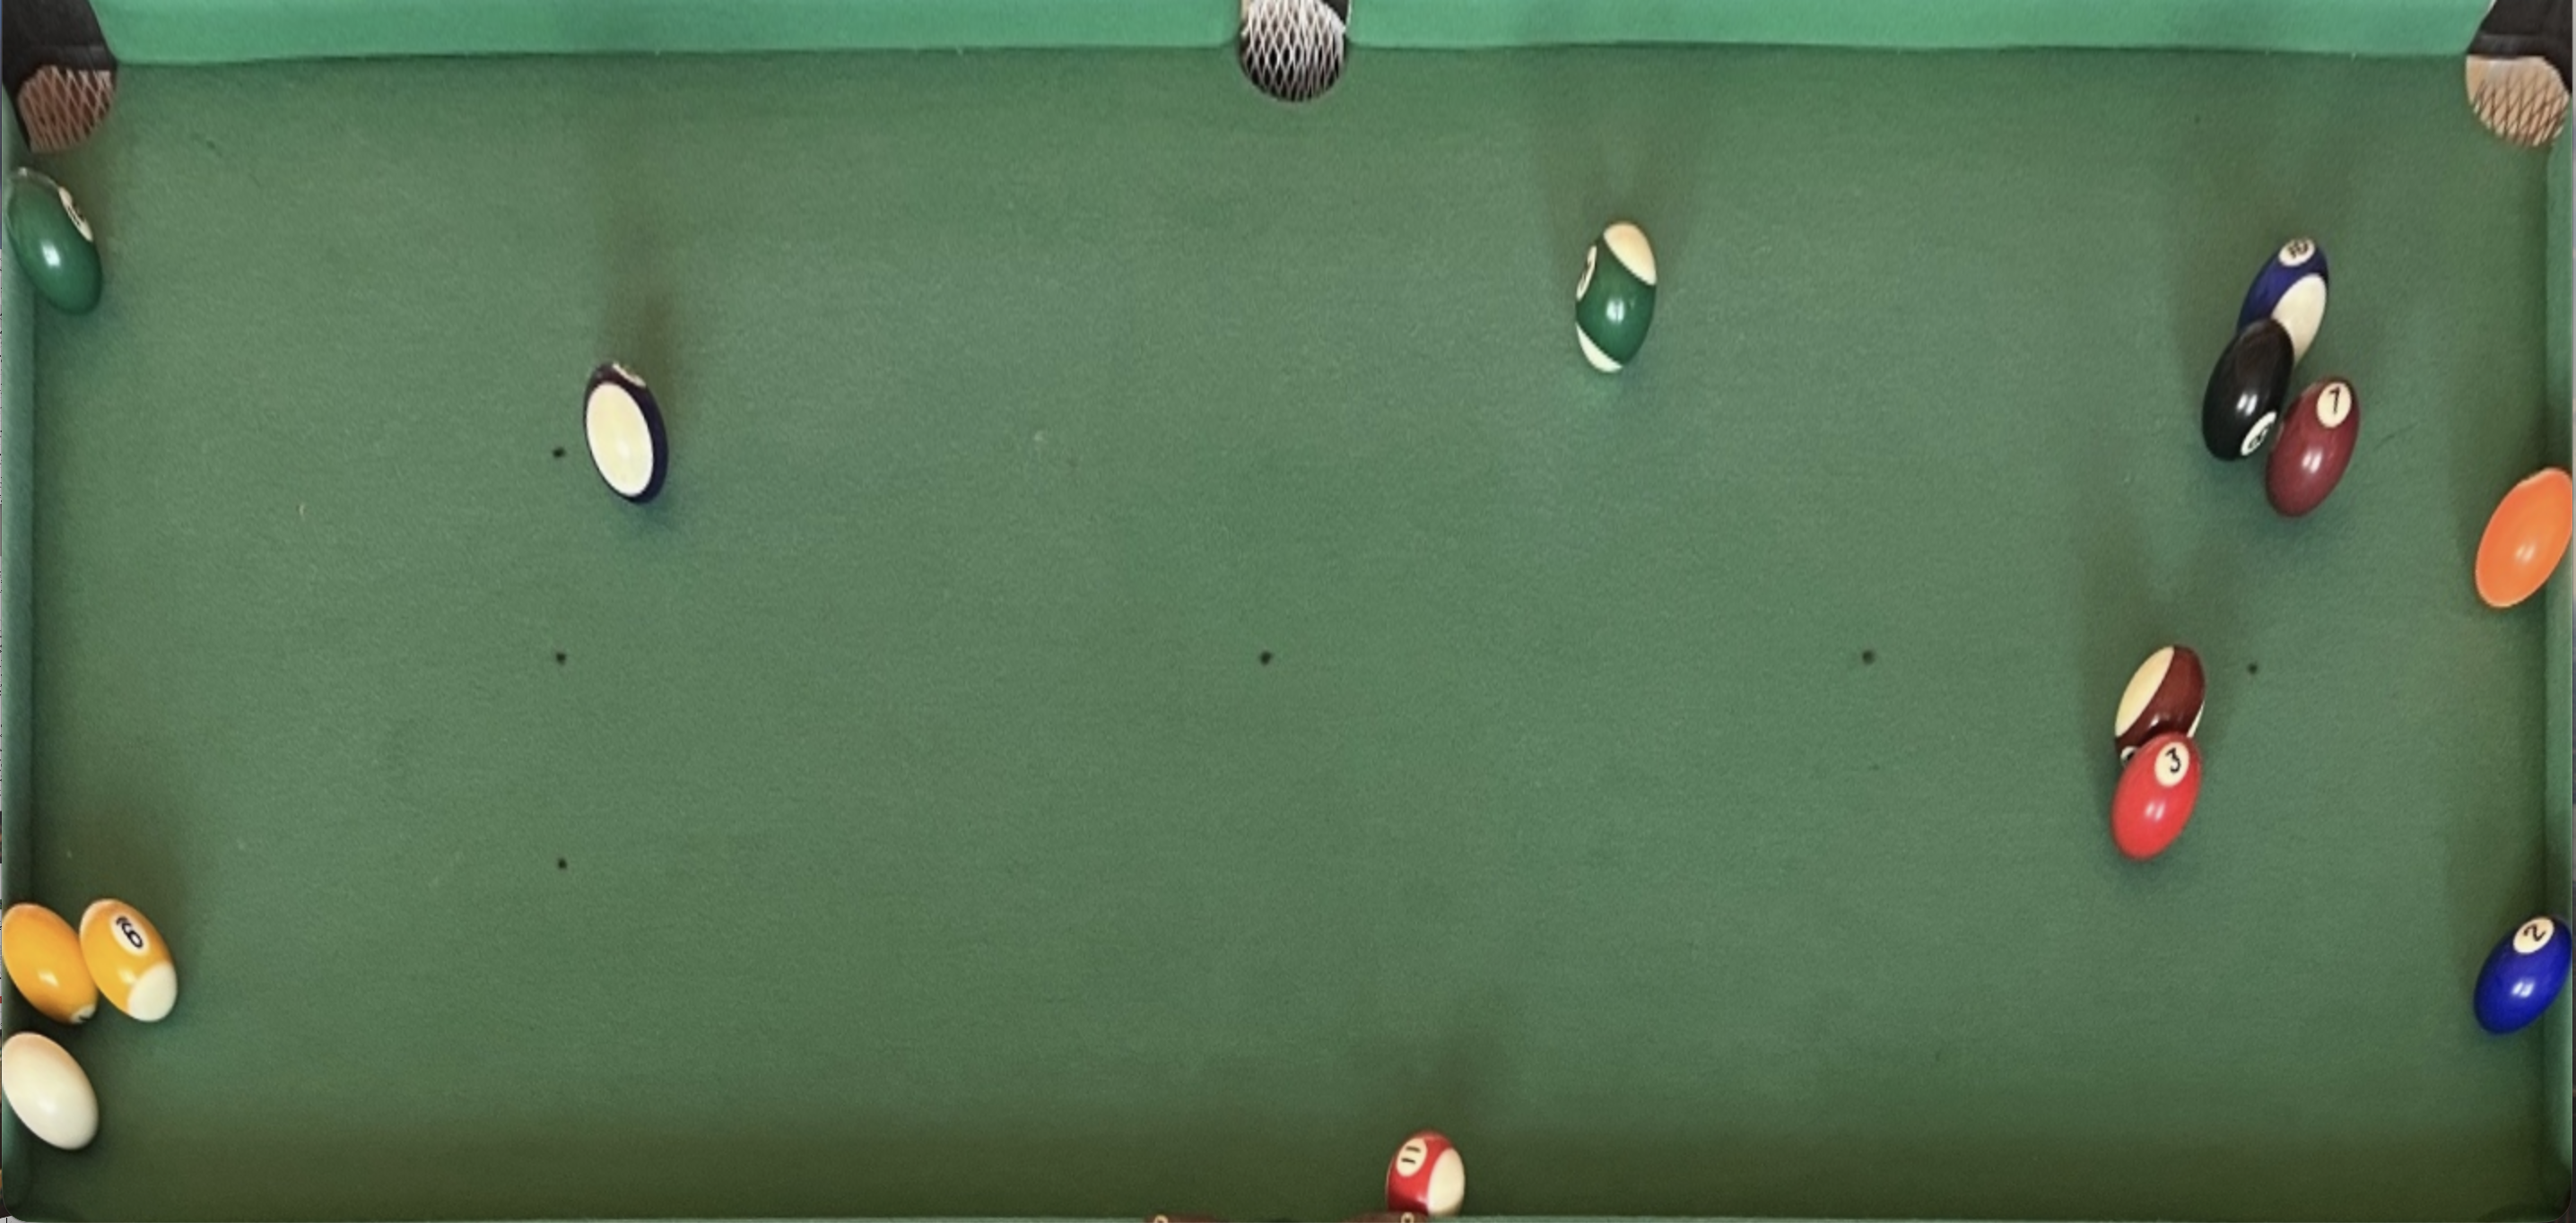
\includegraphics[
            width=\linewidth,
            height=3cm,
            keepaspectratio
        ]{figures/CV_Fig4.png}
        \caption{Training Image with types of balls detected}
        \label{fig:fig3}
    \end{minipage}
    \hfill
    \begin{minipage}[b]{0.6\textwidth}
        \centering
        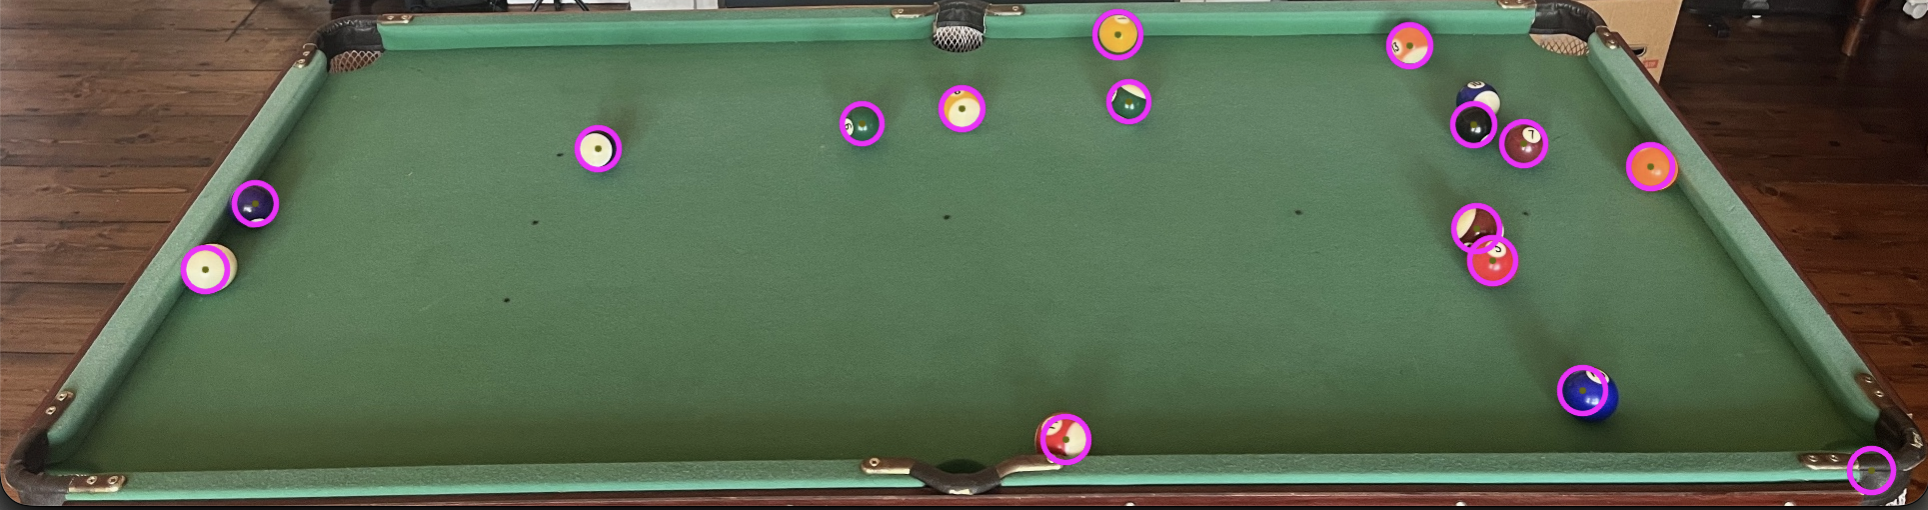
\includegraphics[
            width=\linewidth,
            height=5cm,
            keepaspectratio
        ]{figures/CV_Fig3.png}
        \caption{Hough Circle Transform applied to Table3.jpeg}
        \label{fig:fig4}
    \end{minipage}
\end{figure}

A greedy algorithm was used to determine whether the balls were correctly found or not. Ground truths were used to determine whether a ball was found. The greedy algorithm uses the Euclidean distance formula:
\begin{center}
    $d = \sqrt{(x_2 - x_1)^2 + (y_2 - y_1)^2}$
\end{center}
where $x$ are the coordinates for the ground truth centers and $y$ are the coordinates for the detected circle. The detected circles' centre coordinates were transformed into the same geometric space as the ground truths to ensure accuracy. The transformation allows for 1mm $\approx 1$ pixel. The algorithm would match the balls after they were detected. It would go through all available ground truth coordinates and find the ground truth coordinate that has the smallest distance with the detected ball, provided that it also is less than the distance limit of 23 pixels. This limit was chosen as each pool ball is roughly 43mm in diameter, and once transformed, it would be $\approx43$ pixels. In order to account for cases where the centre of a ball might lie on the edge of another ball, the limit was 22 pixels.

\subsection{Recognising the pool balls}
The recognition implementation involved using HSV classification thresholds and K-means clustering to find the main colour within the ball to determine what ball it was. This allows for the main colours within the image to be found, using the Blue, Green, Red (BGR) colour space. 
BGR allows for colours across all three channels to be considered for recognising the ball. Hue, Saturation and Value (HSV) was also used to help find the white and black pixels to help determine the white, black, striped and solid coloured balls. 
A training image, "AllBalls.jpeg" was used to find the different thresholds for HSV and K-means clustering. The image was transformed geometrically to get a top-down view of the pool table as it would allow for balls to be more similar in size, making the area for the colour recognition to be more consistent. 
K was set to 3 as it would create clusters for the coloured pixels within the ball and uses the dominant cluster. The centre of the circle along with 4 points on the circle's circumference were transformed geometrically to find a circle mask to fit the transformed balls. 
The radius of the ball was reduced to 90\% of the transformed radius, as to try and remove any background pixels. 
However, it could also cause issues such as parts of the ball not being included in mask. 
A boundary rectangle was created to limit the search area for the pixels while only pixels within the mask were counted for the clusters. 
The saturation and value were used to determine if a pixel was saturated, black, white or a coloured pixel. 
Percentage of white, black and coloured pixels along with mean saturation and mean brightness were used for thresholding. 
These threshold values were set using experimentation to see what produced the correct classification. 
If the ball is solid or striped, K means clustering was performed on all coloured pixels from the ball, provided there was at least 3 coloured pixels, or else it used all the pixels within the mask. 
The cluster with the most amount of coloured pixels was used to classify BGR values to create a reference vector to hold the BGR values for each colour, which was automatically stored.
\begin{figure}[H]
    \centering
    \begin{minipage}[b]{0.4\textwidth}
        \centering
        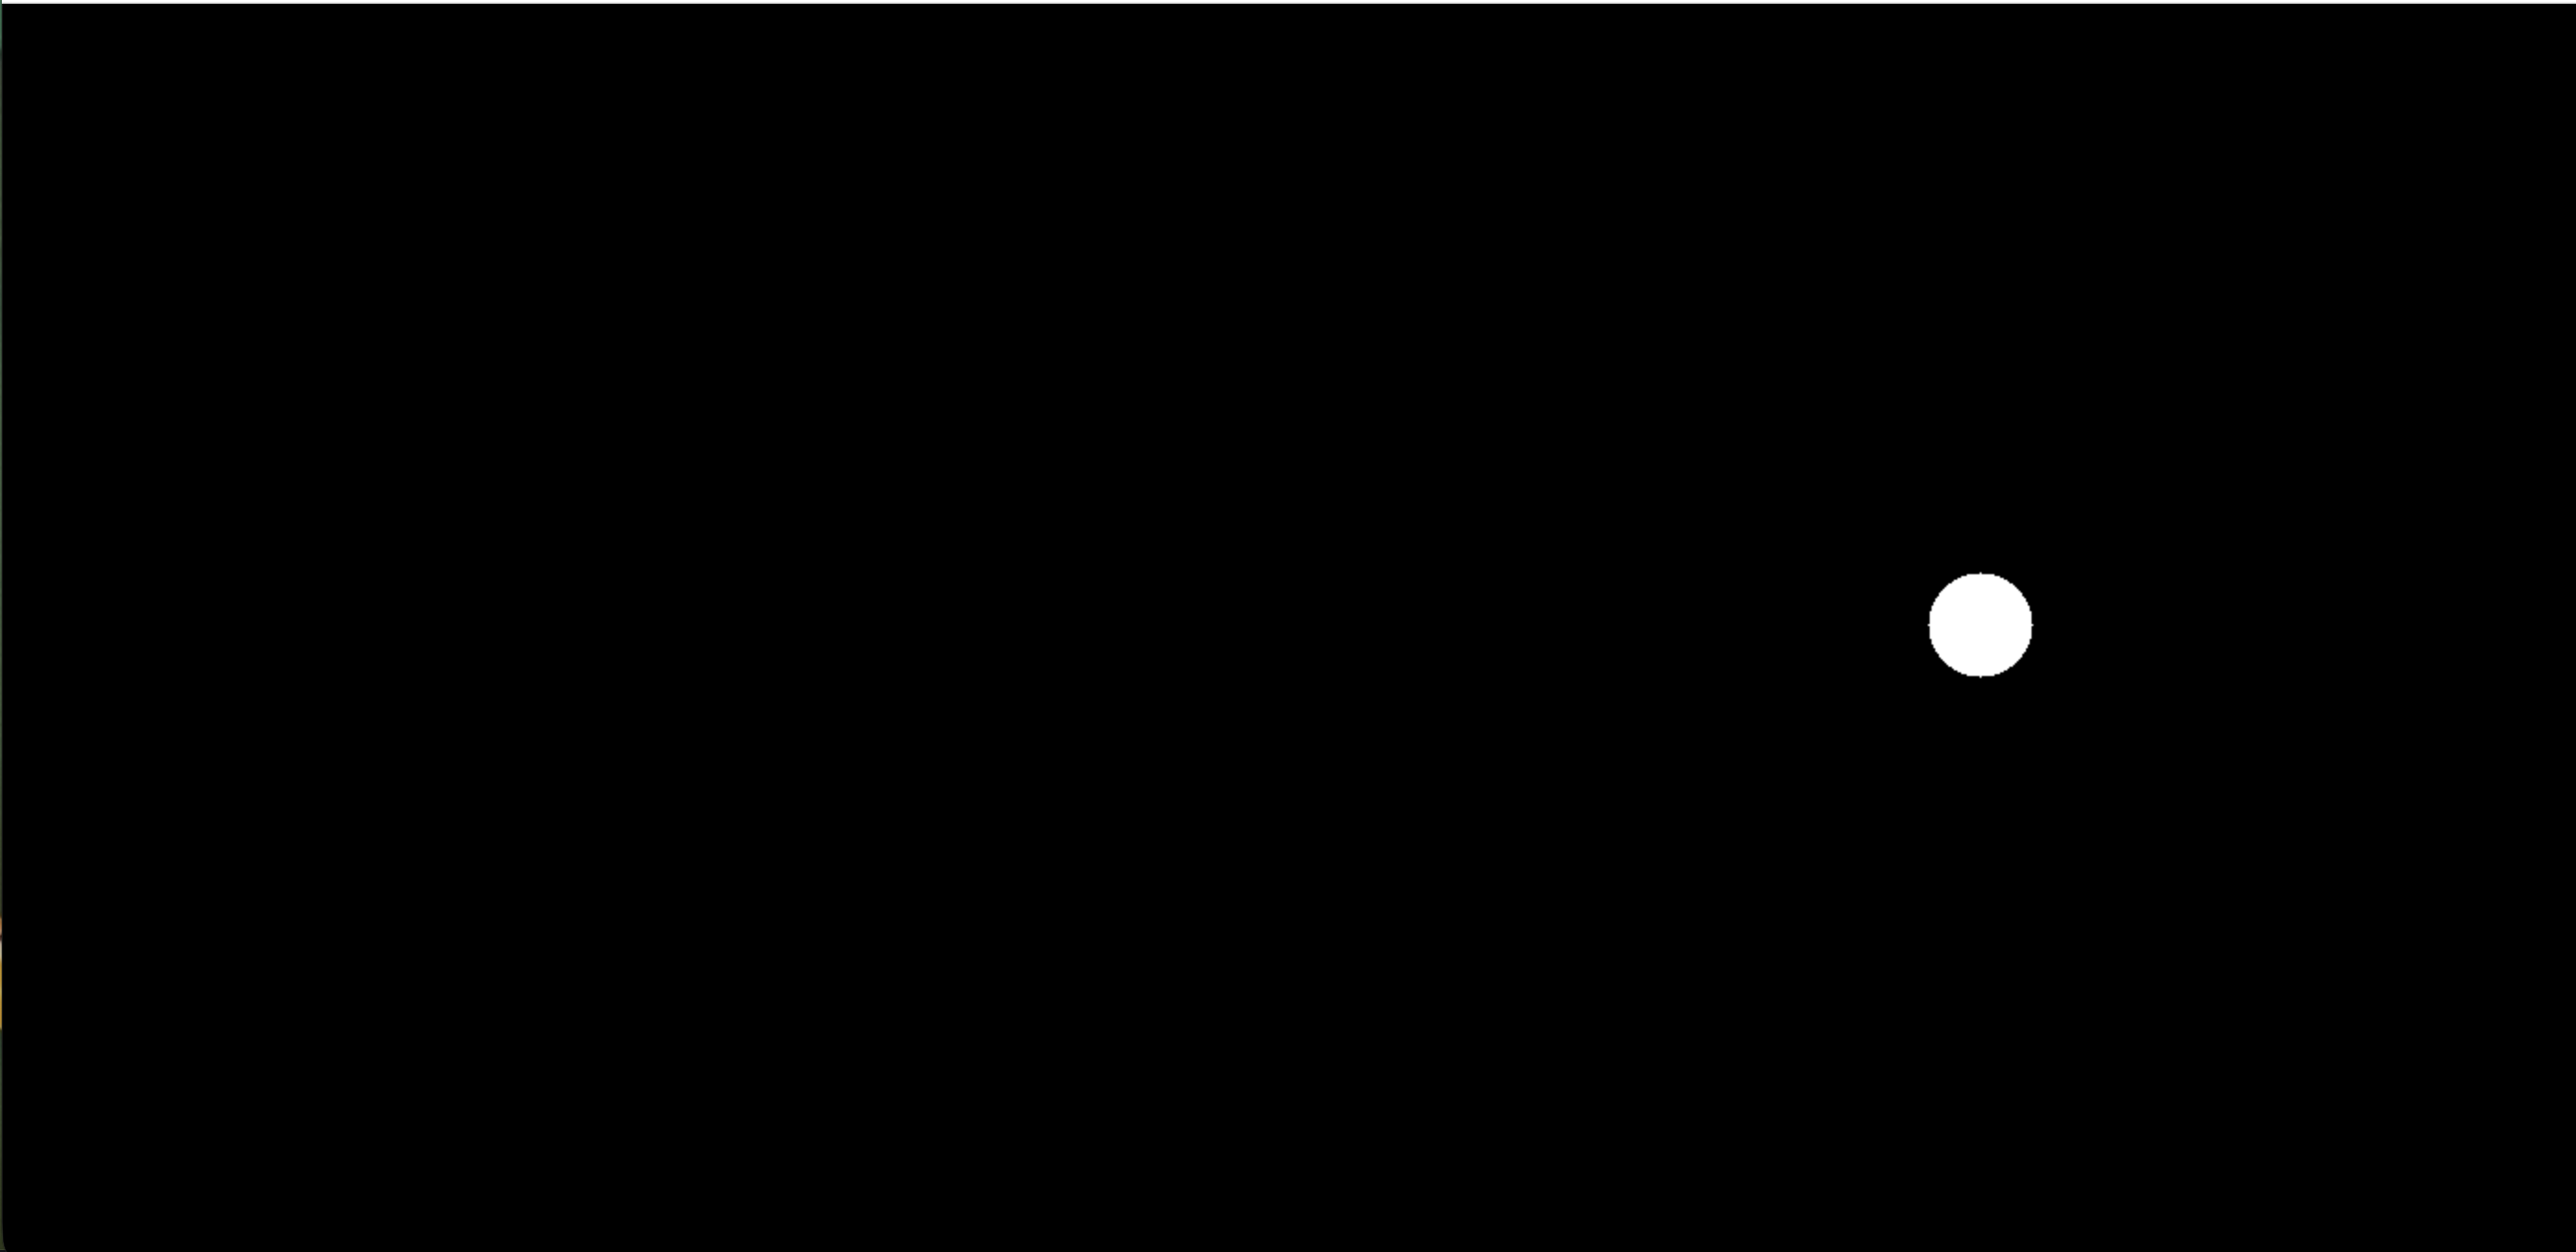
\includegraphics[
            width=\linewidth,
            height=3cm,
            keepaspectratio
        ]{figures/CV_Fig5.png}
        \caption{Mask of the Purple Striped Ball fromAllBalls.jpeg}
        \label{fig:fig3}
    \end{minipage}
    \hfill
    \begin{minipage}[b]{0.4\textwidth}
        \centering
        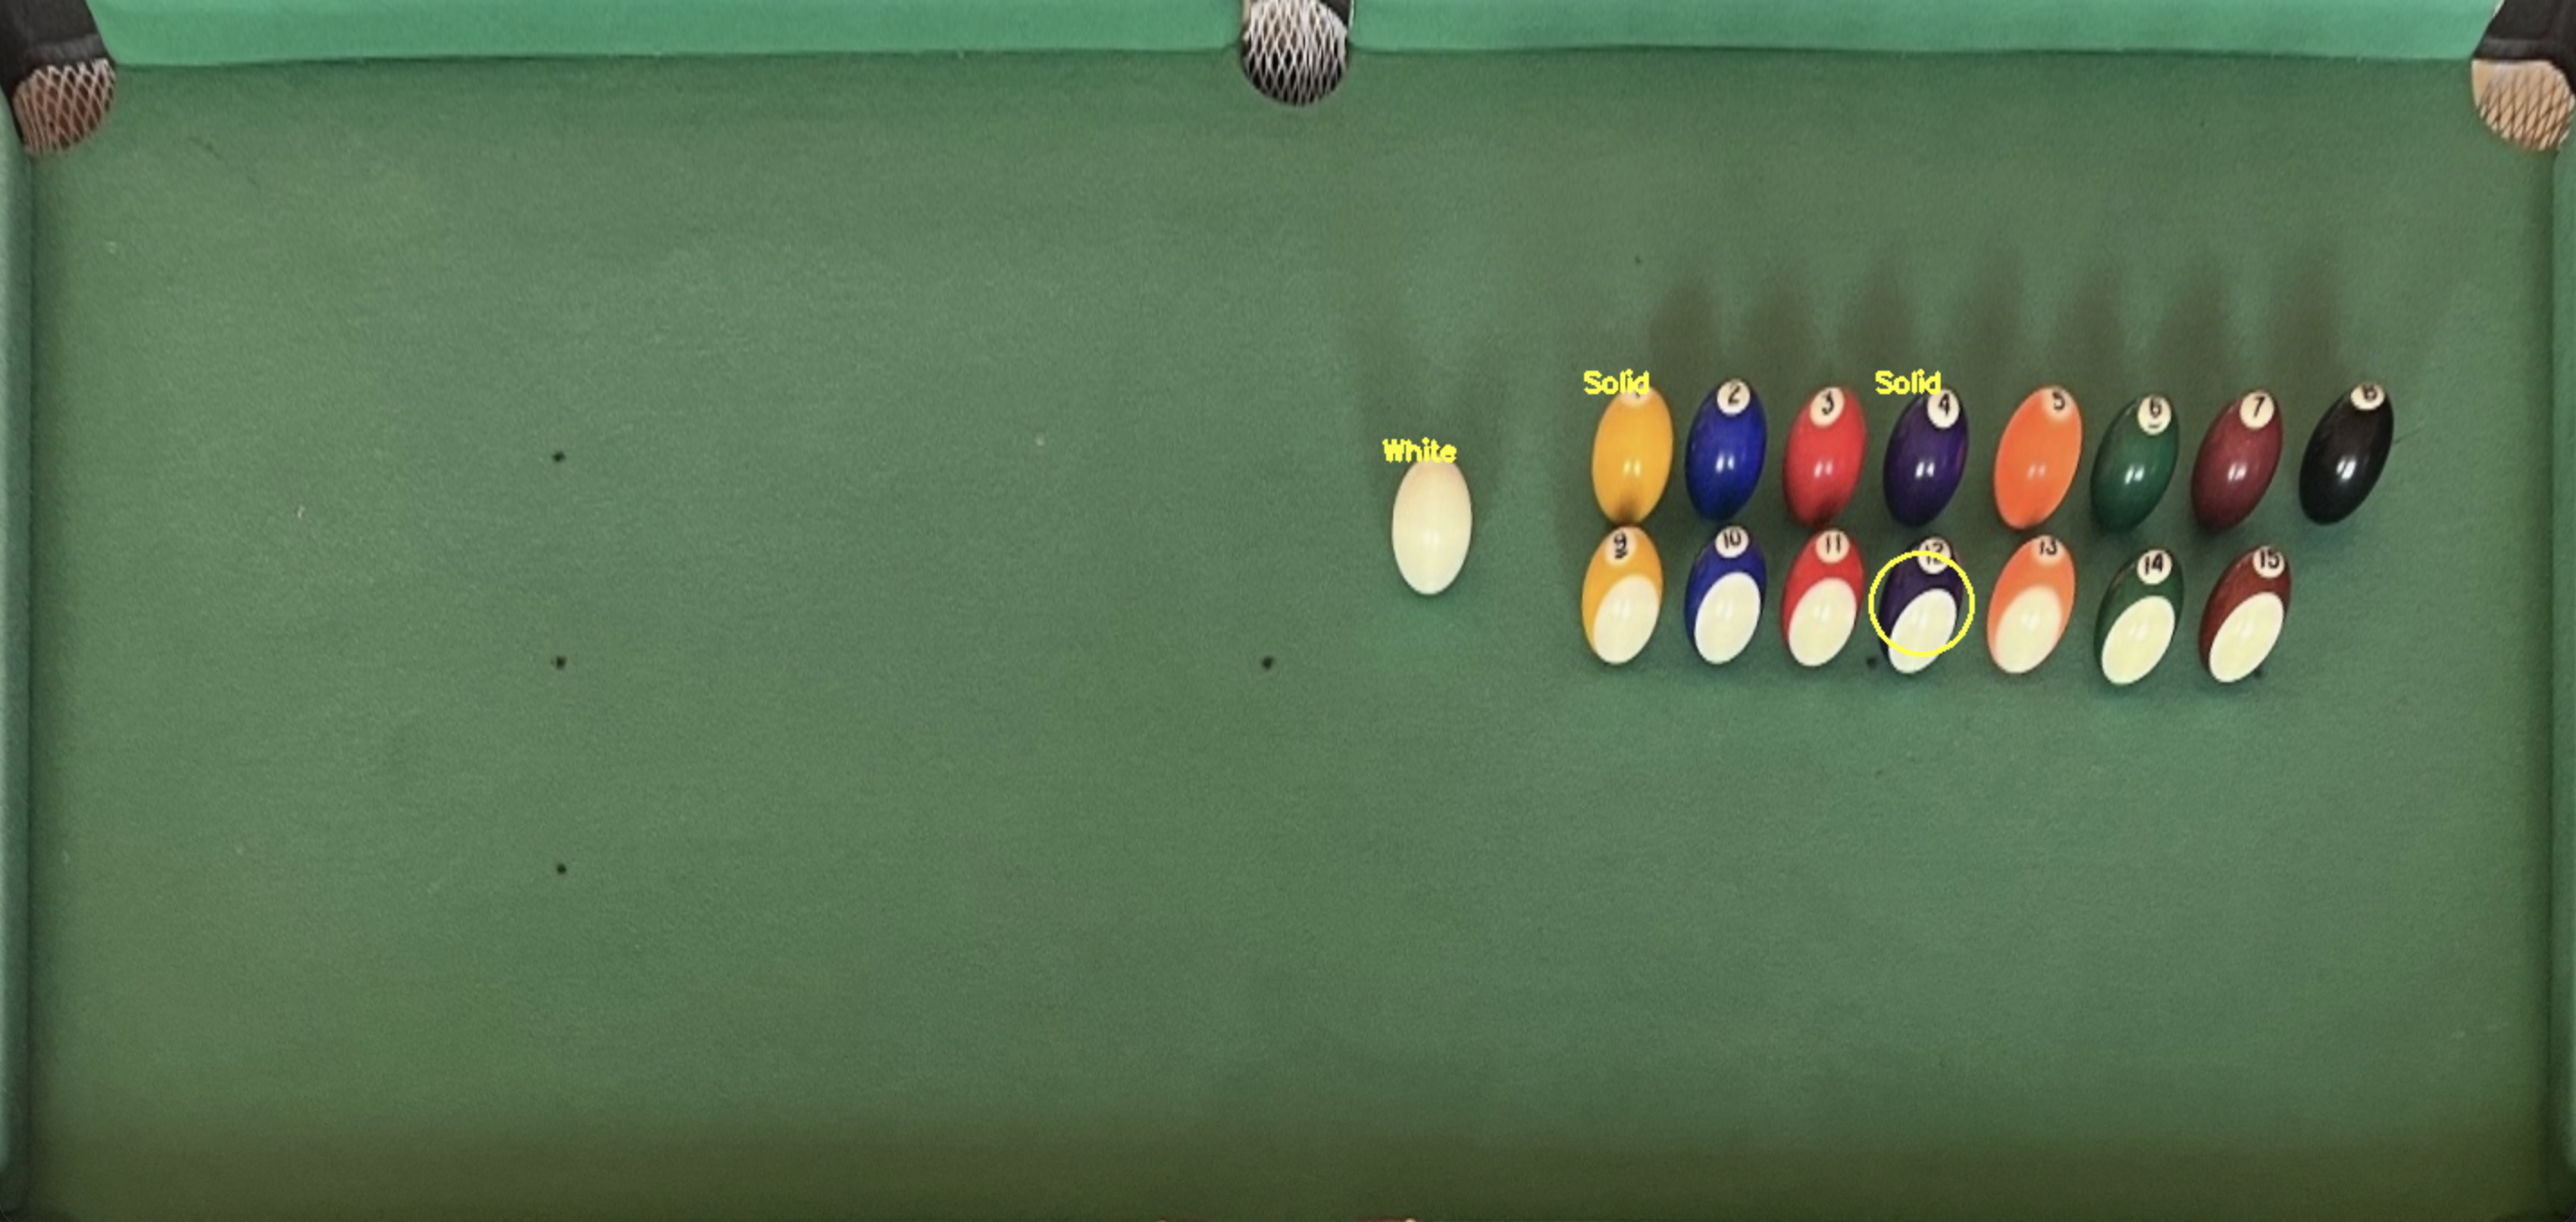
\includegraphics[
            width=\linewidth,
            height=3cm,
            keepaspectratio
        ]{figures/CV_Fig6.png}
        \caption{Mask Area of the Purple Striped Ball on the training image}
        \label{fig:fig4}
    \end{minipage}
    \hfill
    \begin{minipage}[b]{0.4\textwidth}
        \centering
        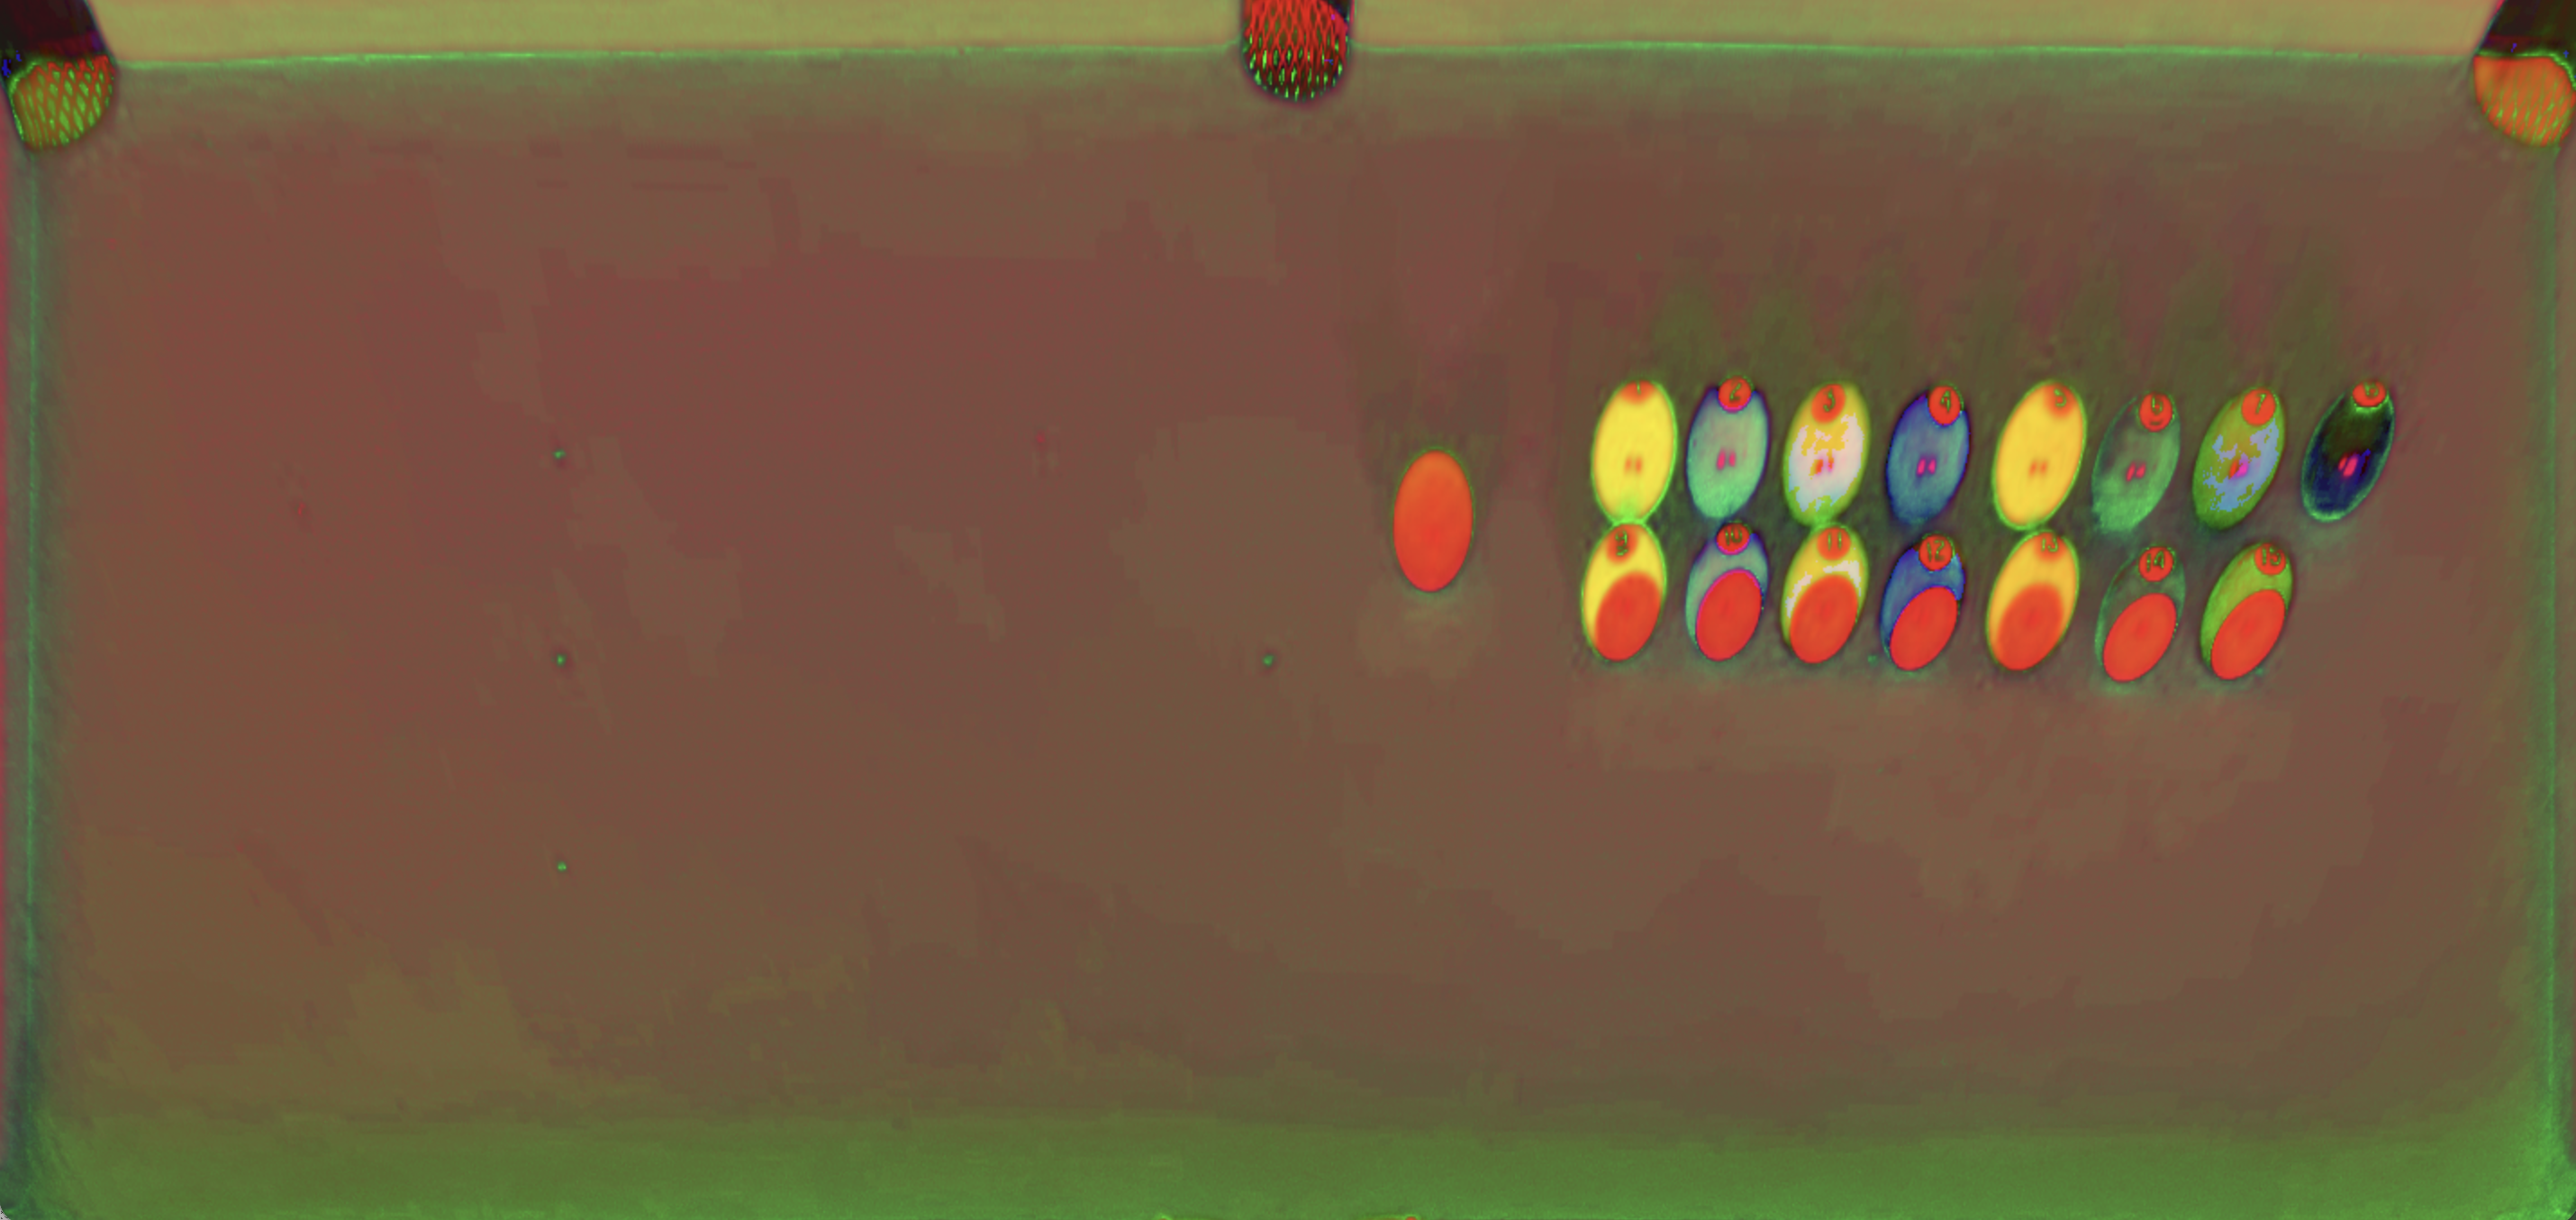
\includegraphics[
            width=\linewidth,
            height=3cm,
            keepaspectratio
        ]{figures/CV_Fig16.png}
        \caption{HSV Image of the training image}
        \label{fig:fig5}
    \end{minipage}
\end{figure}
For the testing images, the same process is repeated for each image. The balls were first classified as white, black, solid or striped using the set thresholds. In order to determine the colour of the balls, the BGR values of the largest cluster was compared with the reference colours from the training image. The comparison used the Euclidean distance formula to computed the distance between the dominant BGR value and each of the references' BGR values and keeps the one with the least amount of distance.
\begin{center}
$d = \sqrt{(B_1 - B_2)^2 + (G_1 - G_2)^2 + (R_1 - R_2)^2}$
\end{center}
$B_1, G_1, R_1$ are values from the dominant cluster and $B_2, G_2, R_2$ are the values from the reference vector. This allows for the nearest colour match of each coloured pool ball. The balls were labeled with 0-15, with 0 being the white cue ball and the other balls with their true number, and any balls that were not recognised were labeled with $-1$. 
\begin{figure}[H]
    \centering
    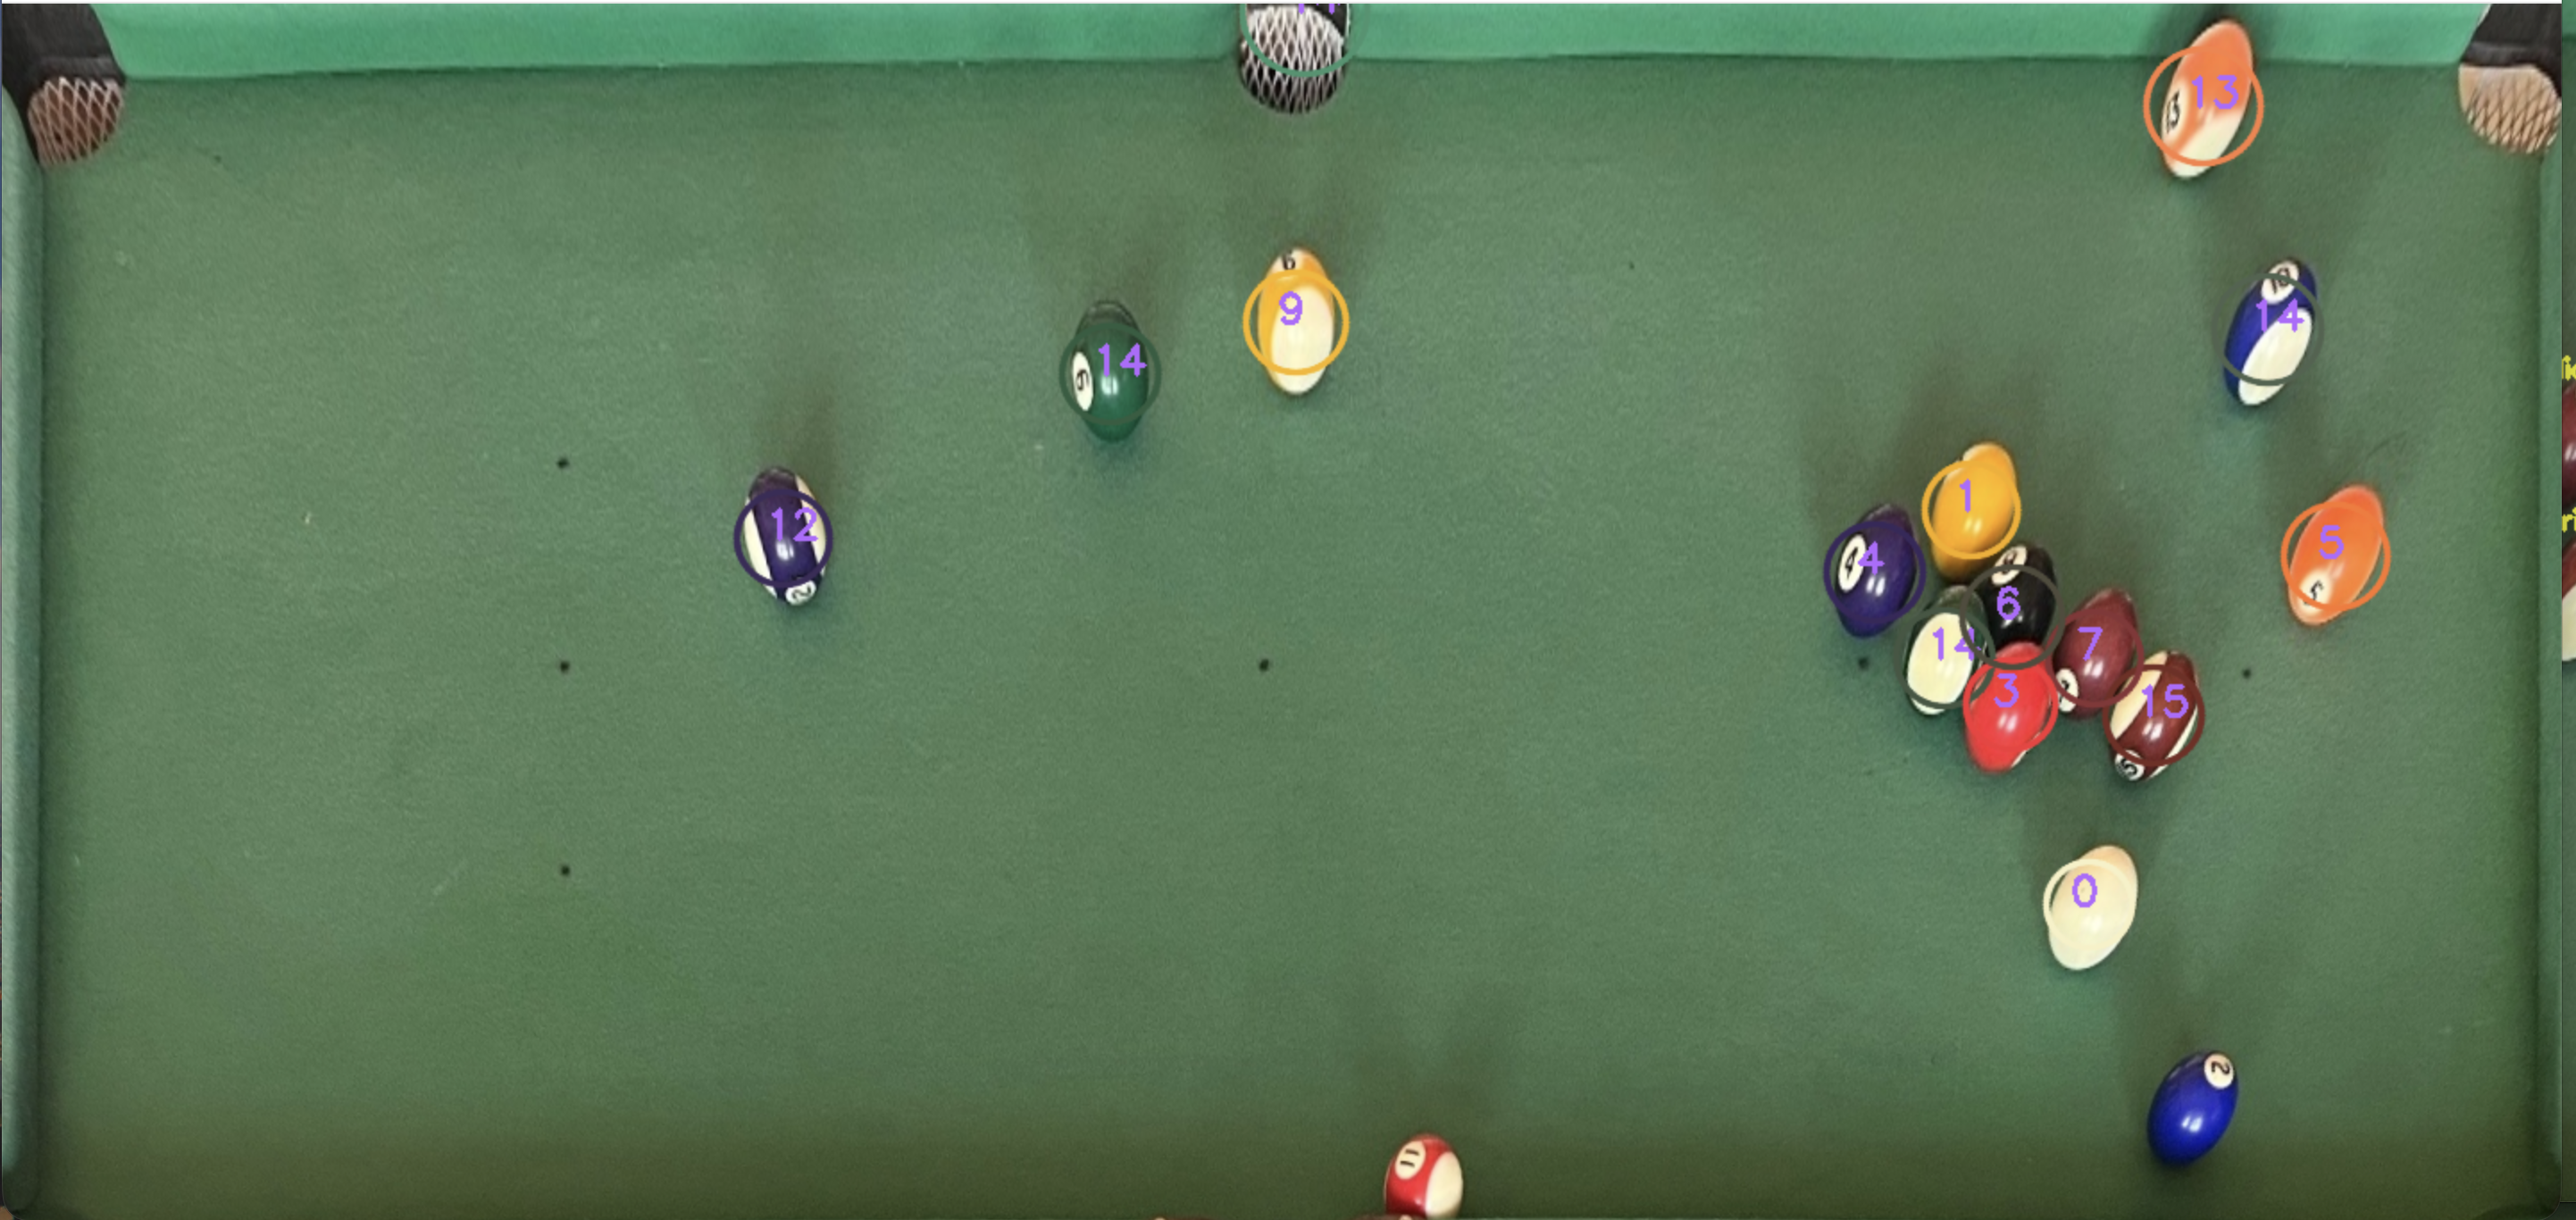
\includegraphics[width=0.5\textwidth]{figures/CV_Fig17.png} 
    \caption{Colour Detection on Table2.jpeg}
    \label{fig:fig_1}
\end{figure}

\section{Results and Analysis}
\subsection{Detecting the pool balls}
The ground truths used to evaluate the methods used were corrected from originally given. They were implemented in order to see how accurate the methods truly are and not how accurate they were against untrue data. 
The results from the matching algorithm for detecting the pool balls were collected using false positives (FP), false negatives (FN) and true positives (TP). A true positive detection had to be a centre detected within the distance limit (23) of a ground truth centre. A false negative is when a ball that was present in the ground truth but the ball was not detected by the Hough Circle Transform. A false positive was recorded when the Hough Circle Transform detected a ball but it was not present in the ground truth. A confusion matrix was not used in evaluating the detection as what could be considered a true negative is unclear. It could consider every pixel that is not a detected centre and not a ground truth centre a true negative, which seemed excessive. Precision, recall and F1 score were used to evaluate the algorithm. Precision measures the amount of predicted positive results that are actually positive. Recall is the amount of true positive result that were correctly predicted [2]. F1 score is the balance between precision and recall [3]. They were calculated as follows:
\[
Recall = \frac{TP}{TP + FN}
\quad
Precision = \frac{TP}{TP+FP}
\quad
F1 \ Score = \frac{2TP}{2TP + FP + FN}
\]
\begin{table}[H]
    \centering
    \begin{tabular}{|c|c|c|c|c|c|c|c|}
    \hline
        Image & TP & FP & FN & Precision & Recall & F1 Score \\
        Table1 & 12 & 0 & 4 &  100\% & 75\% & 85.71\% \\
        Table2 & 14 & 1 & 2 &  93.33\% & 87.5\% & 90.32\%\\
        Table3 & 15 & 1 & 1 &  93.75\% & 93.75\% & 93.75\% \\
        Table4 & 13 & 0 & 2 &  100\% & 86.67\% & 92.86\% \\
        Table5 & 12 & 1 & 2  & 92.31\% & 85.71\% & 88.89\% \\
        Table6 & 12 & 0 & 1 &  100\% & 92.31\% & 96\% \\
        \hline
        Overall Average & 13 & 0.5 & 2 & 96.57\% & 86.82\% & 91.26\% \\
        \hline
    \end{tabular}
    \caption{Detection Metric Results for each Image}
    \label{tab:placeholder}
\end{table}

From the table above, the detection performs relatively well. Table6 performed the best. It has the highest F1 score of 96\% and it had no false positives and only 1 false negatives. Table1 has the worst detection, with 4 false negatives, meaning it missed four balls on the table. This is most likely due to the balls being clustered together, making it harder to detect the circles. The overall average precision score is $96.57\%$, meaning $\approx97\%$ of the predicted positive detections were actual positive detections. The overall average recall score was $86.82\%$, meaning $\approx 87\%$ of the ground truth centres were correctly predicted. The average F1 score was $91.26\%$, or $\approx 91\%$. This indicates the Hough Circle Transform performs quite well on detecting the balls. One issue is that some of the balls do not get detected when they are covered by others. A way to improve on this might be to use watershed segmentation as it could distinguish between balls that touch or overlap within the image, allowing for the borders to be seen using watershed lines.
Another issue is that the pockets of the table sometimes get detected as a ball. This is most likely due to the circular shape of the pocket. One way to remove this error could be to use contour segmentation to find holes within the Hough Circles and if a certain number of holes are found, like the holes in the pocket netting, it is considered a pocket and thus ignored.
\begin{figure}[H]
    \centering
    \begin{subfigure}[b]{0.6\textwidth}
        \centering
        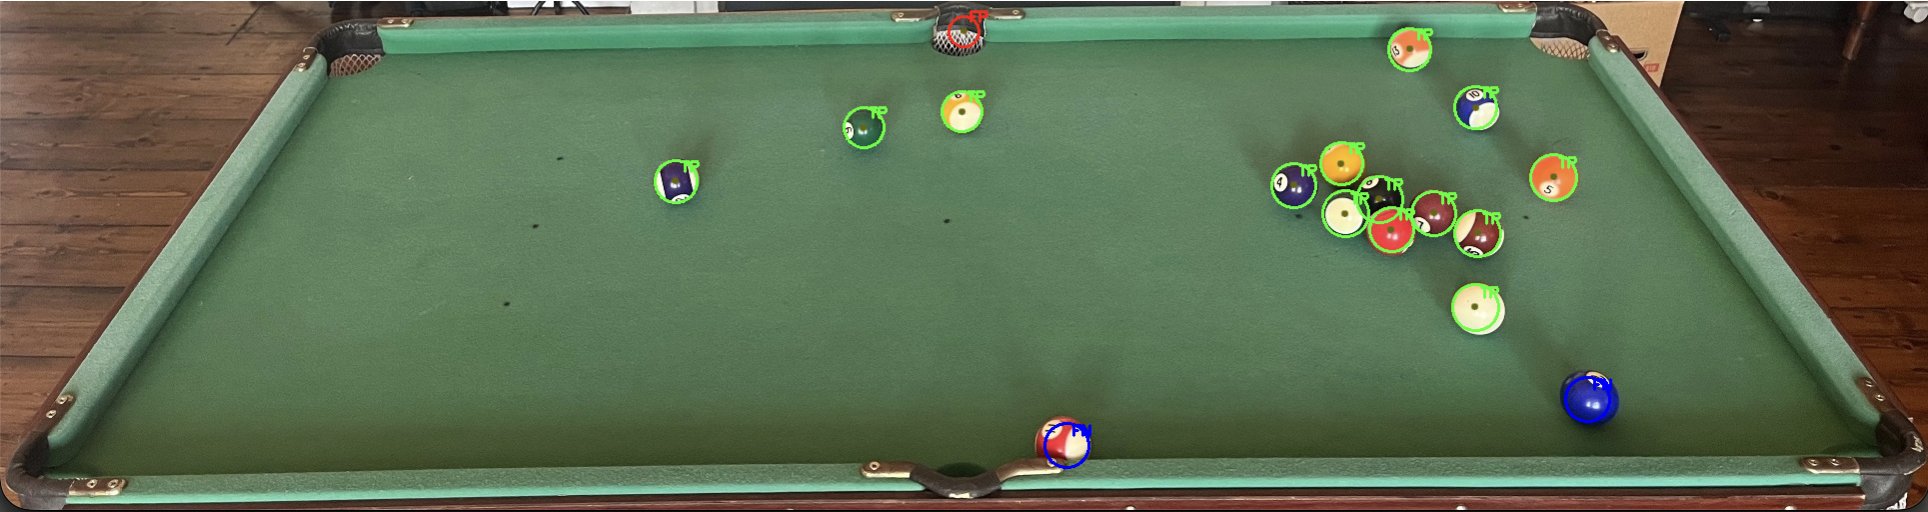
\includegraphics[width=\linewidth]{figures/CV_Fig8.png}
        \caption{Detection on Table2.jpeg}
        \label{subfig:a}
    \end{subfigure}%
    \\
    \begin{subfigure}[b]{0.6\textwidth}
        \centering
        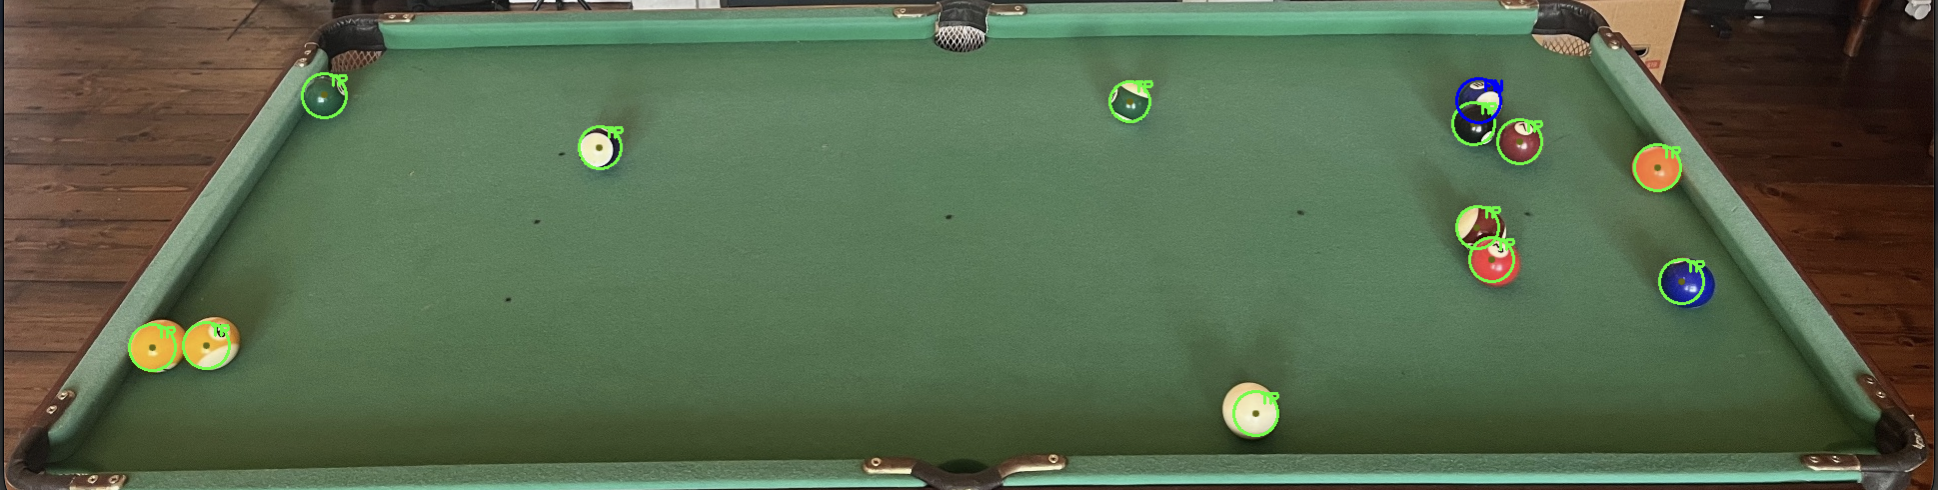
\includegraphics[width=\linewidth]{figures/CV_Fig9.png}
        \caption{Detection on Table6.jpeg}
        \label{subfig:b}
    \end{subfigure}%
    \caption{Hough Circle Transform detection, true positives denoted in green, false negatives in blue and false positives in red}
    \label{fig:ball_masks}
\end{figure}

\subsection{Recognising the pool balls}
The recognition of the balls was evaluated using a confusion matrix, and associated metrics: accuracy, precision, recall, specificity, and F1 score. A confusion matrix presents the true positive, true negative, false positive and false negative values recorded from the recognition. In order to gauge just the recognition, without the influence of the detection, the confusion matrix was generated using only detected balls that had a successful ground truth match. It does not include missed balls. A true positive is when a certain ball was correctly recognised, a false positive is when a different ball was recognised as the certain ball, a true negative is when the ball being recognised was not recognised as a different colour  and a false negative is when the certain ball was recognised as a different colour. Precision, recall and F1 score was calculated in the same way as for detection. Accuracy is how well the recognition performed overall [2] and specificity is  how well the recognition could identify true negatives [4] was calculated using the folllowing formulas:
\[
Accuracy = \frac{TP+TN}{TP + FN + TN + FP}
\quad
Specificity  = \frac{TN}{TN + FP}
\]
\begin{table}[H]
\centering
\label{tab:recognition_metrics}
\resizebox{\textwidth}{!}{%
\begin{tabular}{|l|c|c|c|c|c|c|c|c|c|}
\hline
\textbf{Ball Number and Type} & \textbf{TP} & \textbf{FP} &
\textbf{TN} & \textbf{FN} & \textbf{Accuracy} &
\textbf{Precision} & \textbf{Recall} &
\textbf{Specificity} & \textbf{F1 Score} \\

\hline
Ball 0: White & 5 & 0 & 72 & 1 & 98.72\% & 100\% & 83.33\% & 100\% & 90.91\% \\
\hline
Ball 1: Yellow Solid & 6 & 0 & 72 & 0 & 100\% & 100\% & 100\% & 100\% & 100\% \\
\hline
Ball 2: Blue Solid & 3 & 0 & 74 & 1 & 98.72\% & 100\% & 75\% & 100\% & 85.71\% \\
\hline
Ball 3: Red Solid & 6 & 0 & 72 & 0 & 100\% & 100\% & 100\% & 100\% & 100\% \\
\hline
Ball 4: Purple Solid & 3 & 0 & 75 & 0 & 100\% & 100\% & 100\% & 100\% & 100\% \\
\hline
Ball 5: Orange Solid & 5 & 1 & 71 & 1 & 97.44\% & 83.33\% & 83.33\% & 98.61\% & 83.33\% \\
\hline
Ball 6: Green Solid & 2 & 1 & 72 & 3 & 94.87\% & 66.67\% & 40\% & 98.63\% & 50\% \\
\hline
Ball 7: Brown Solid & 4 & 0 & 73 & 1 & 98.72\% & 100\% & 80\% & 100\% & 88.89\% \\
\hline
Ball 8: Black & 4 & 0 & 73 & 1 & 98.72\% & 100\% & 80\% & 100\% & 88.89\% \\
\hline
Ball 9: Yellow Striped & 5 & 1 & 71 & 1 & 97.44\% & 83.33\% & 83.33\% & 98.61\% & 83.33\% \\
\hline
Ball 10: Blue Striped & 0 & 1 & 75 & 2 & 96.15\% & 0\% & 0\% & 98.68\% & 0\% \\
\hline
Ball 11: Red Striped & 3 & 0 & 75 & 0 & 100\% & 100\% & 100\% & 100\% & 100\% \\
\hline
Ball 12: Purple Striped & 1 & 0 & 72 & 5 & 93.59\% & 100\% & 16.67\% & 100\% & 28.57\% \\
\hline
Ball 13: Orange Striped & 4 & 1 & 73 & 0 & 98.72\% & 80\% & 100\% & 98.65\% & 88.89\% \\
\hline
Ball 14: Green Striped & 5 & 5 & 67 & 1 & 92.31\% & 50\% & 83.33\% & 93.06\% & 62.50\% \\
\hline
Ball 15: Brown Striped & 5 & 2 & 71 & 0 & 97.44\% & 71.43\% & 100\% & 97.26\% & 83.33\% \\
\hline
\end{tabular}}
\caption{Recognised Balls Confusion Matrix Metrics}
\end{table}
The recognition of the balls generally performs well. The accuracy for each ball is quite high, with the lowest being the Green striped ball at $92.31\%$. However, accuracy is not a true indication of performance as the number of true negatives skews the accuracy to be much higher. This is also the same for specificity as it uses true negatives in its calculation. Precision, recall and F1 score are more accurate indications of the recognition's performance. For example, the Blue Striped Ball has an accuracy of $96.15\%$, yet it does not actually correctly recognise a Blue Striped ball. This is seen by the precision, recall and F1 score each being $0\%$. The recognition struggles to identify the Green Solid, Blue Striped, Purple Striped and Green Striped balls. The Purple Striped ball often gets labelled as "-1", meaning that it is unable to be classified by the sytem. This could be resolved by using more training data in order to get a more accurate analysis of the pixels in the Purple Striped ball. Some of the balls have $100\%$ in precision, recall and F1 score, such as the Red Striped, Red Solid, Yellow Solid and Purple Ball. As the recognition only considers matched detected balls that were recognised, it can overestimate how successful it is at recognising the balls as some balls that were not detected and matched were not considered. 

\subsection{Overall detection and recognition}
The overall detection and recognition was calculated using a confusion matrix, with similar metrics as the previous two anaylsis. However, true negatives were not included in the overall metrics as previously said, the pool ball detection method cannot accurately determine what is a true negative. A true positive is a corrected detected and recognised ball. A false positive is a ball that was incorrectly recognised or the detection was not matched with a ground truth. A false negative was a ball incorrectly recognised or missed during detection. The overall evaluation focused on precision, recall and F1 score, using the same calculations as before. 
\begin{table}[H]
    \centering
    \begin{tabular}{|c|c|c|c|c|c|c|c|}
    \hline
         TP & FP & FN & Precision & Recall & F1 Score \\
        61 & 20 & 29 & $75\%$ & $68\%$ & $71\%$ \\
        \hline
    \end{tabular}
    \caption{Overall detection and recognition evaluation metrics }
    \label{tab:placeholder}
\end{table}
Overall, the detection and recognition performs relatively well. The precision is at $75\%$, meaning that $75\%$ of detected and recognised balls were true positives. The recall score means that $68\%$ of actual true balls were correctly detected and recognised. The F1 score means the balance between detected and recognised balls being true and true balls being detected and recognised was $71\%$. This is quite good, yet does leave room for improvement. 

The detection method was tuned and the recognition method was tuned on one image, AllBalls.jpeg. This means that the parameters for the Hough Circle Transform, the white, dark, coloured and saturated percentages of the different types of balls and the colour references were all dependent on one image. If the method would be used on images in a different lightning settings or at a different angle, it might not perform as well. A larger training dataset would be beneficial to help the algorithms perform better. If other objects were on or near the pool table such as a pool cue or a person leaning over the table to shoot, they could block balls from view, preventing them from being detected and recognised. The greedy algorithm used also only matches a detected ball and its ground truth as it sees it and does not optimally match the balls. This can lead to misclassification of the balls.


\section{Final Result Images}

\begin{figure}[H]
    \centering
    \begin{subfigure}[b]{0.5\textwidth}
        \centering
        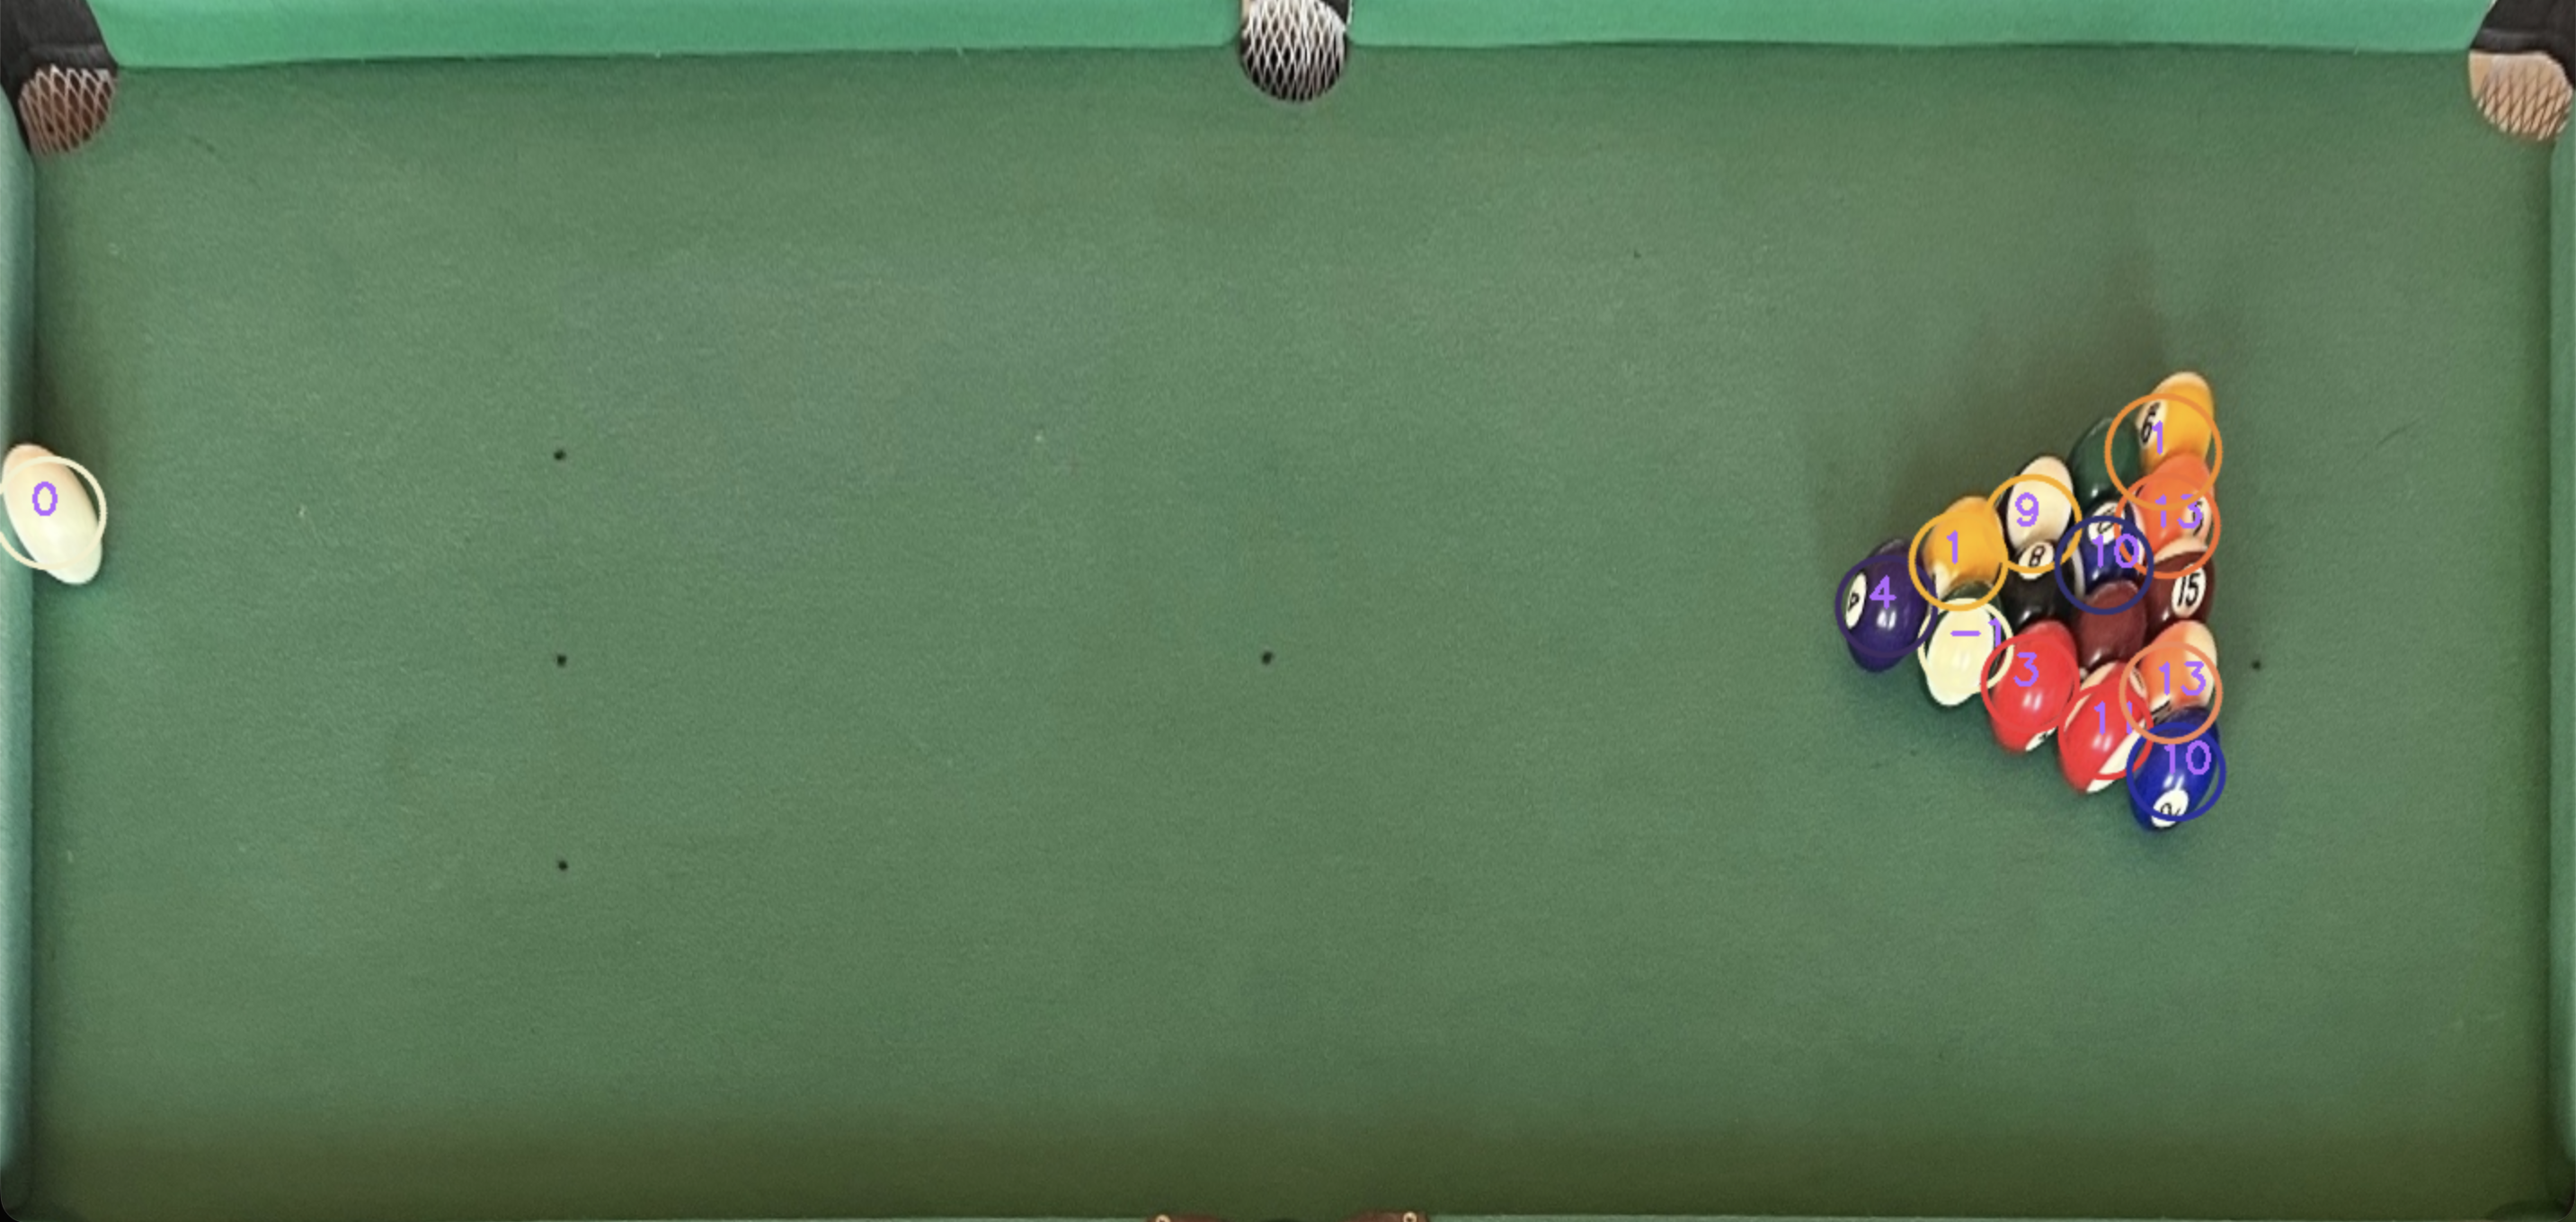
\includegraphics[width=\linewidth]{figures/CV_Fig10.png}
        \caption{Table1.jpeg}
        \label{subfig:a}
    \end{subfigure}%
    \\
    \begin{subfigure}[b]{0.5\textwidth}
        \centering
        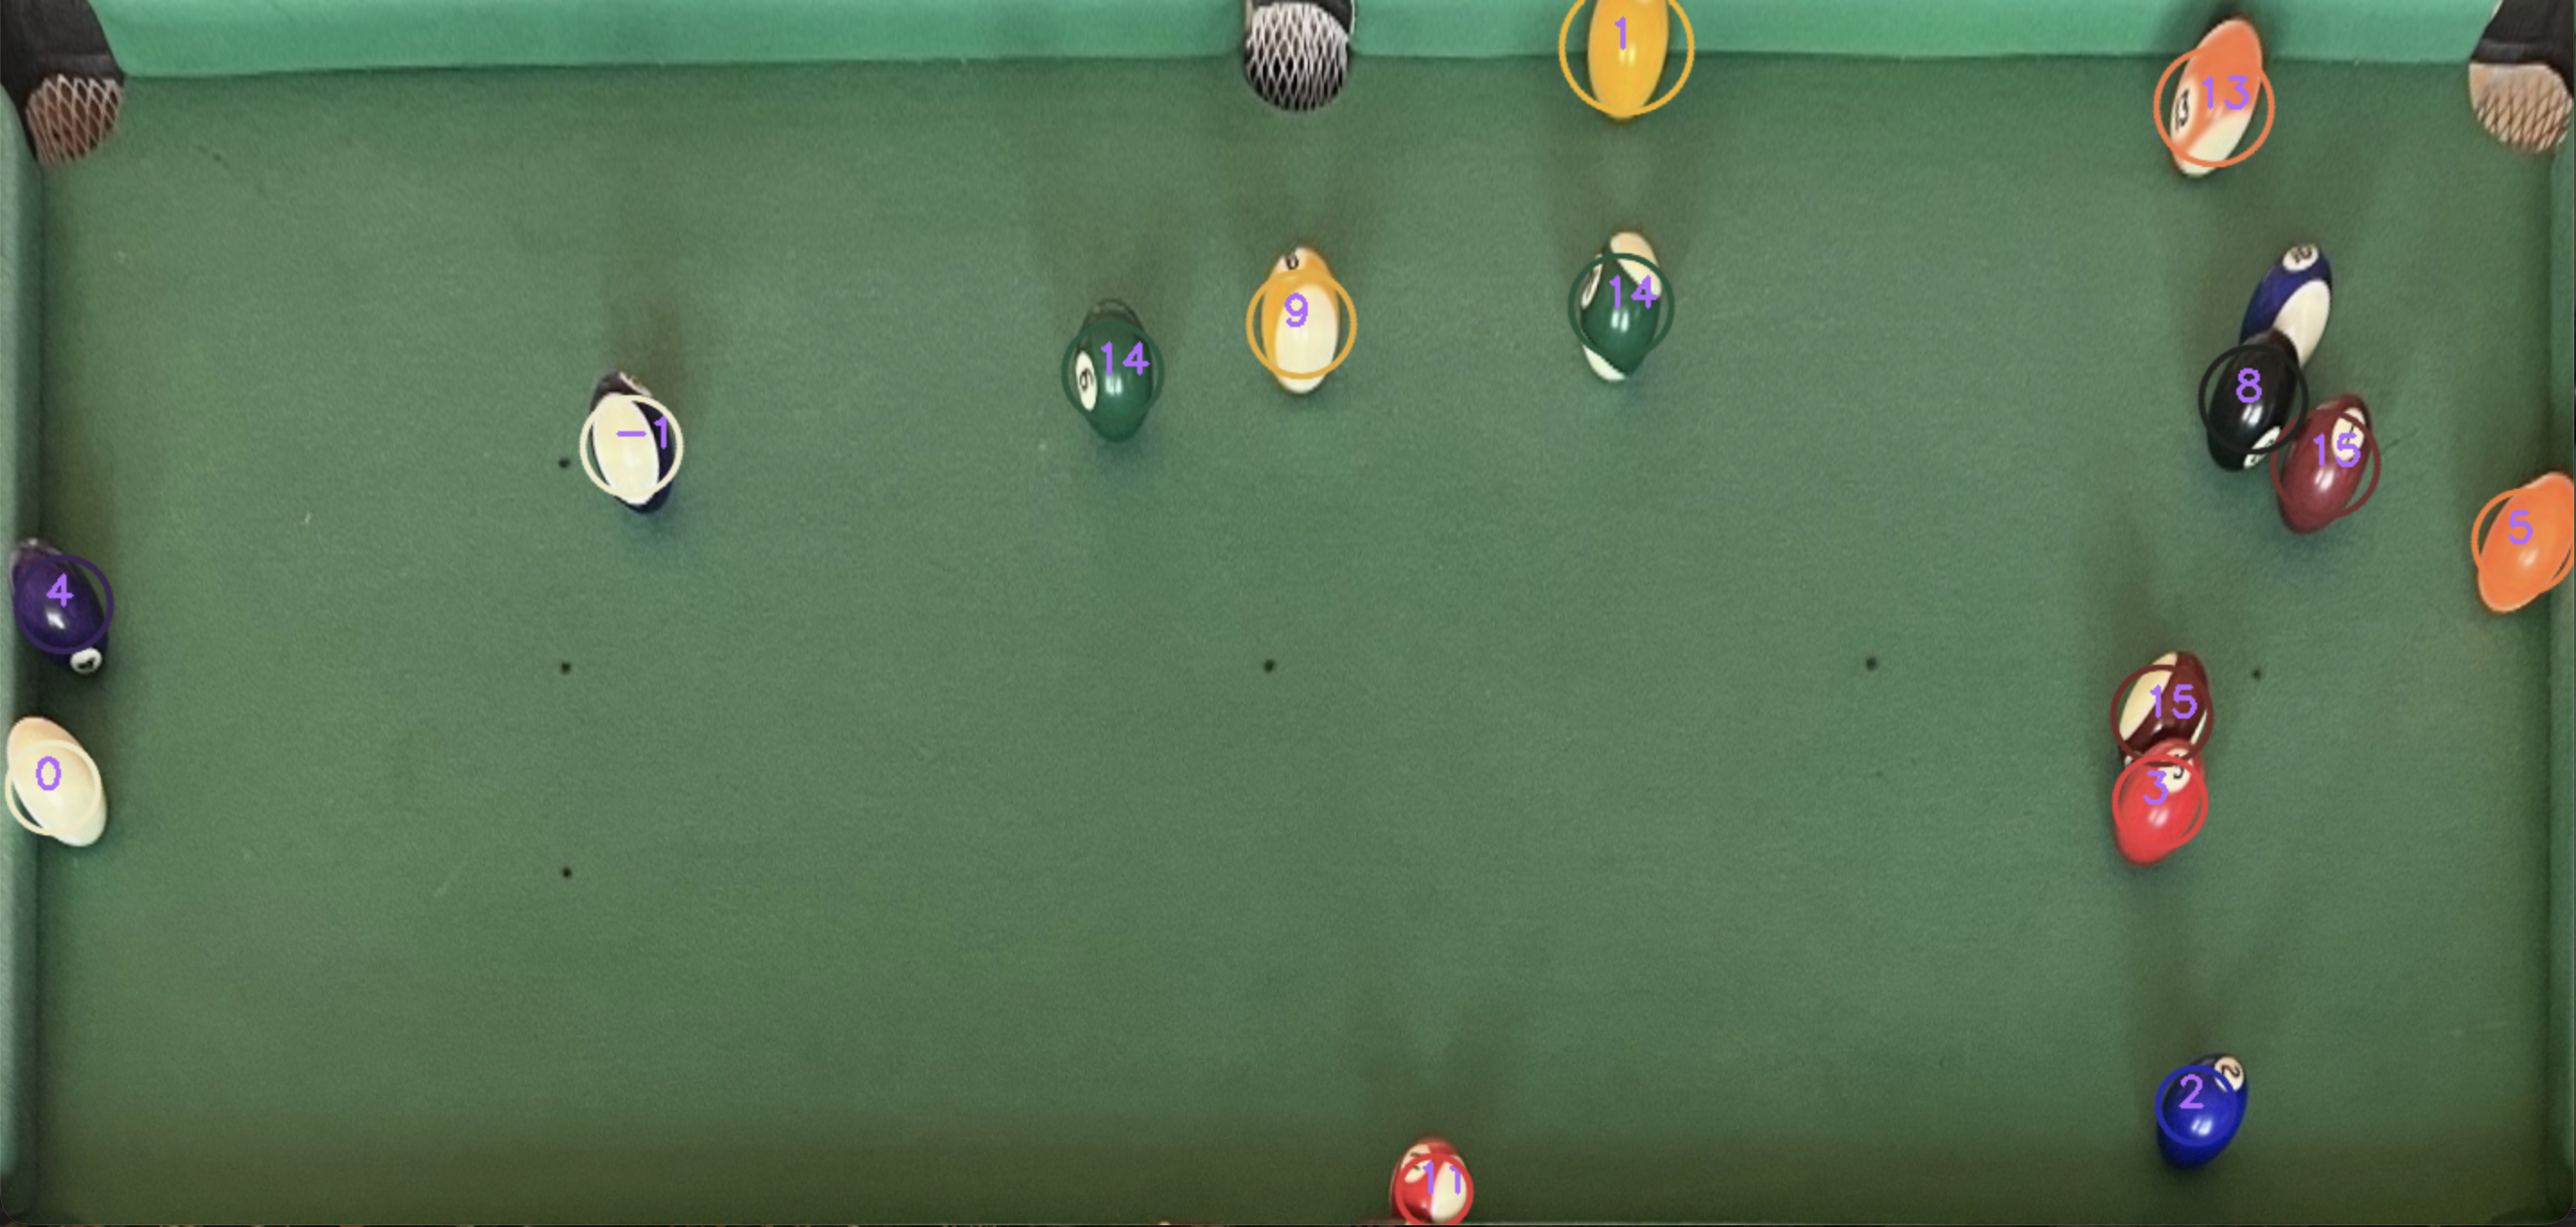
\includegraphics[width=\linewidth]{figures/CV_Fig12.png}
        \caption{Table3.jpeg}
        \label{subfig:a}
    \end{subfigure}%
    \\
    \begin{subfigure}[b]{0.5\textwidth}
        \centering
        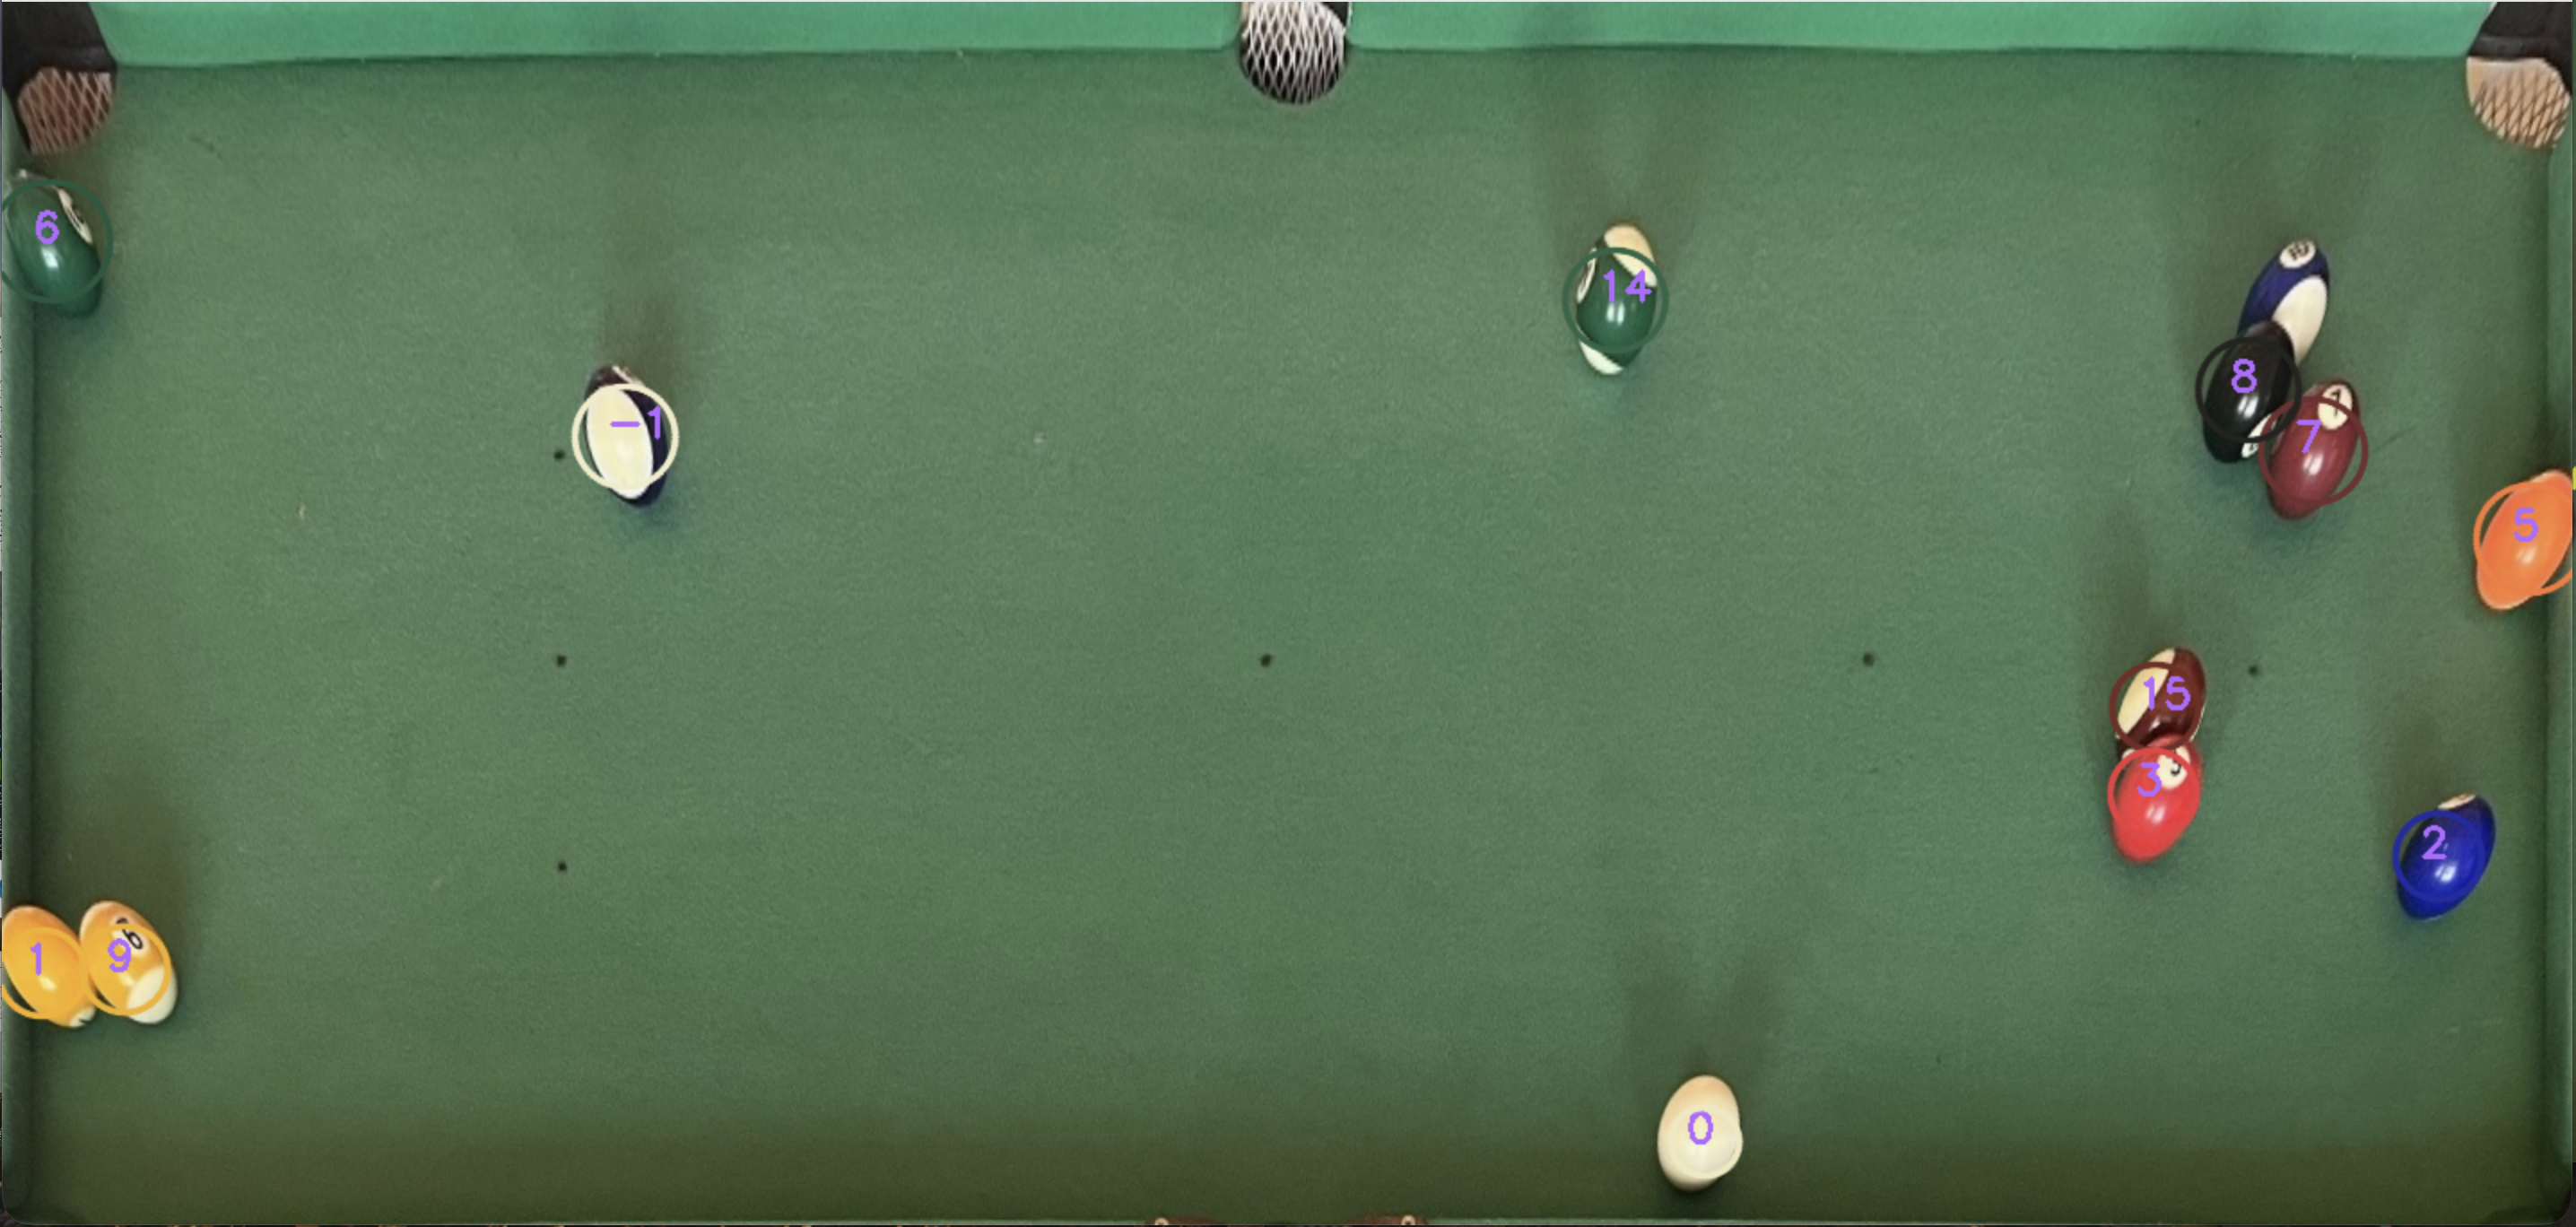
\includegraphics[width=\linewidth]{figures/CV_Fig15.png}
        \caption{Table6.jpeg}
        \label{subfig:b}
    \end{subfigure}%
    \label{fig:ball_masks}
\end{figure}


\section{References}
1. Feature Detection, OpenCV, 2025, \\
\url{https://docs.opencv.org/4.13.0/dd/d1a/group__imgproc__feature.html#ga47849c3be0d0406ad3ca45db65a25d2d}
\\
2. Classification: Accuracy, recall, precision, and related metrics, Google Developers, 2026, \url{https://developers.google.com/machine-learning/crash-course/classification/accuracy-precision-recall}
3. F1 Score in Machine Learning, Geeks for Geeks, 2026, \url{https://www.geeksforgeeks.org/machine-learning/f1-score-in-machine-learning/}\\
4. Understanding the Confusion Matrix in Machine Learning, Geeks for Geeks, 2026, \url{https://www.geeksforgeeks.org/machine-learning/confusion-matrix-machine-learning/}\\
5. CSU44053, Computer Vision Slides, Dr Kenneth Dawson-Howe, Trinity College Dublin.
\end{document}
